
\documentclass{graduation}
\usepackage[dvipdfmx]{graphicx}
\usepackage{epsf}
\usepackage{url}
\usepackage{amsmath}
\usepackage{amsfonts}
\usepackage{float}
\usepackage{indentfirst}
\makeindex
%----------------------------------------------
\begin{document}

\title{
機械学習を用いた\\
変形ARマーカの位置姿勢推定
}
%\etitle{}
\author{ER17076 安井 理}
%\eauthor{}
\date{2021年2月12日} %(卒業研究発表会の日時とする)
\university{中部大学}
\school{工学部ロボット理工学科}
\degree{2020年度 卒業}
\prof{山内 悠嗣}

\frontmatter
\maketitle

%----------------------------------------------
\setcounter{page}{1}
\chapter*{はじめに}
\label{chap:introduction}
現在QRコードやARマーカなどの2次元コードは,製造での工程管理,
製品ピッキング棚卸やロボット認識機能等の広い分野で利用されている.
2次元コードの特徴として,シンボルと呼ばれる特殊なパターンにより,
どの視点からでも背景模様の影響を受けない,高精度な検出が可能である.
さらに2次元コードの大きさを事前に定義することにより,張り付けられている物体の位置,
姿勢を推定することが可能である.ロボットが物体検出を行う時に2次元コード
を使用することなくパターン認識や機械学習を用いた物体検出の研究も取り組まれているが,
画像から物体の検出・姿勢推定を高精度に認識することが困難である.2次元コードを用いた
認識であれば,高速かつ高精度な検出・姿勢推定が可能である.

しかし,2次元コードを使用する前提条件として,
平面に張り付ける事が挙げられる.
この条件以外の,曲面や角に張られた2次元コードは歪みにより見え方の変化を引き起こし,
認識精度が低下する問題を抱えている.2次元コードに歪みを補正する機能はあるが,補正には限界がある.
試しに円柱などの平面でないものに2次元コードを貼り認識を試みると,歪みにより正確に認識ができない場合がある.平面状でない2次元コードの認識は困難であり,この問題を解決するための研究がされている.

そこで,本研究では,Augument Autoencoder(AAE)を用いた変形ARマーカの平面化及び姿勢推定を提案する.変形したARマーカの画像をAAEに入力し,歪みを取り除いた平面状のARマーカ画像を生成する.そして,変形ARマーカの姿勢推定を行う.


本論文の以下の構成は次のようになっている.第 1 章では,2 次元コードの種類と AR
マーカの認識について述べる.第 2 章では,曲面に貼られた変形 AR マーカを機械学習に
より推論し,推論結果を用いて正面から観測した AR マーカー画像を生成する手法を提案
する.第 3 章では,学習データの作成方法について述べる.最後に,第 4 章で評価実験に
ついて述べる.

%----------------------------------------------

%目次の生成
\tableofcontents

%図が無い場合には下記を削除し,図の目次を表示しないようにしてください
\listoffigures
%表が無い場合には下記を削除し,表の目次を表示しないようにしてください
\listoftables


%これ以降のページ番号の書体を変える設定
\mainmatter

%----------------------------------------------
\chapter{ARマーカについて}
\label{chap:1}

本章では,本研究で扱うARマーカを含む2次元コードの概要を示す.

\section{2次元コード}

2次元コードとは,1方向のみに情報を持たない1次元バーコードに対して,水平方向と垂直方向の2方向に情報を持つ事が可能な表示方式のコードである.バーコードと比較をすると記録できる情報量が多くなり,面積当たりの情報密度が高いため,コード化するデータが同一の場合2次元コードの方が表示面積が小さくなる.その為,バーコードは識別コードとして使用される事に対して,2次元コードは大容量データ媒体として使用することが可能である.




\subsection{2次元コードの認識}
2次元コードは主にスタック型2 次元コードとマトリクス型2 次元コードの2種類に分けられる.

\begin{itemize}
\item スタック型2次元コード \\
シンボルキャラクタまたはデータコードワードと呼ばれるバーコードシンボルが情報の基本単位となっている.
行の情報を表したロウインジケータが配置されており,どの行からでも読み込める.スタート・ストップコードに囲まれている.バーコードと同様にバーの幅で情報を表すため,レーザスキャンによる読み込みも原理的に可能である.
スタック型2次元コードの代表例として,PDF417やCODE49などがある.
\end{itemize}

\begin{itemize}
\item マトリクス型2次元コード \\
セルと呼ばれる正方形や点を格子状に配列した構造を持つ2次元コードであり,一般的な外形は正方形である.
2次元コードの位置検出を行うため,正方形の枠やL字のフレームで囲われていたり,ファインダパターンと呼ばれる特徴的なマークがシンボルのなかに配置されている.セルの配置パターンを画像処理によりデコードし,
カメラまたは2次元CCD素子内蔵のリーダで読み込みを行う.
これにより,シンボルの方向に影響されることなく,全方向で読み取ることが可能になる.
マトリクス型2次元コードの代表例として,QR コード,DataMatrixや本研究で使用するARマーカなどがある.
\end{itemize}





\subsection{2次元コードの問題点}
2次元コードには汚れや傷などのデータの欠損に対して,
読み込んだデータを元のデータに復元するリードソロモン法と呼ばれる数学的エラーを検出し訂正する手法を取り入れた,誤り訂正機能がついているものが多くあることから,ある程度の汚れや傷などであれば読み取ることができる.
しかし,変形していたり,汚れや傷などによってデータの欠損が大きくあり,読み取れなかった場合に,1次元のバーコードであればヒューマンリーダブルと呼ばれる手動で入力出来る数字が付与されているが,2次元コードは情報量が多くヒューマンリーダブルを付与することができない.その為,2次元コードは読み取れなかった場合,情報を得ることができなくなってしまうため,2次元コードは正確に読み取る必要性がある.









\section{ARマーカ}
本研究で使用するARマーカについて説明する.
ARマーカには,「マーカタイプ」,「マーカレスタイプ」,「GPSタイプ」の3種類に分けられる.

\newpage


\begin{itemize}
\item マーカタイプ \\

1つ目の「マーカタイプ」とはマーカを必要とするもので,実際にARマーカを張り付けカメラに写して使うタイプである.ARマーカにはイラストや写真をマーカとして使用することもできるが,色や境界線がはっきりとしないと精度が落ちてしまうため,正方形の黒枠に囲まれた白黒の図\ref{マーカ}に示すような図形が一般的である.
黒枠でARマーカであると認識し,枠内の図柄のパターンでマーカの区別を行う.
本研究ではマーカタイプのARマーカを使用し実験を行った.
      \begin{figure}[htpp]
      \begin{center}
      
\includegraphics[width=40mm]{figure/eps/ARマーカ.eps}
      \caption{ARマーカ.}
      \label{マーカ}
      \end{center}
      \end{figure}


\end{itemize}



\begin{itemize}
\item マーカレスタイプ \\



2つ目の「マーカレスタイプ」は基本的な機能はマーカタイプと同様であるがマーカを必要としないことが特徴である.物理的にマーカが配置できない場合でも情報を付加できることが魅力であるが,計算量がおおきくなってしまいハードウェアに一定の能力が必要となる.そのため専門的な知識も必要になり技術的な難易度が高い. 


\end{itemize}


\begin{itemize}
\item GPSタイプ \\


3つ目の「GPSタイプ」はGPSを用いて場所に応じて不可情報を加えるものである.GPSなどの位置情報だけでなく磁気センサや加速度センサなども併用することで情報やサービスを提供する場所やタイミングを決めている.しかし,GPSの機能やGPSを受け取る端末の性能の精度により影響を受けてしまうため,環境によっては誤差が生じてしまう可能性がある.



\end{itemize}















%----------------------------------------------

%----------------------------------------------
\chapter{機械学習を用いた姿勢推定}
\label{chap:2}
本章では,姿勢推定の従来法の説明をする.


\section{6次元物体検出}
6次元の物体検出は,3次元空間座標だけでなく物体のroll,pitch,yawの3次元姿勢情報を含んだ検出問題である.
高速に推定を行えることに加え,6次元の姿勢情報を持つ教師データがなくても学習可能な手法である.
6次元の姿勢情報を持つ教師データの代わりに,検出対象となる物体の3D CADデータを使用する.
6次元物体検出における,全体の処理の流れを図\ref{fig:2d_pose_estimation}\cite{AAE}に示す.
      \begin{figure}[htbp]
      \begin{center}
      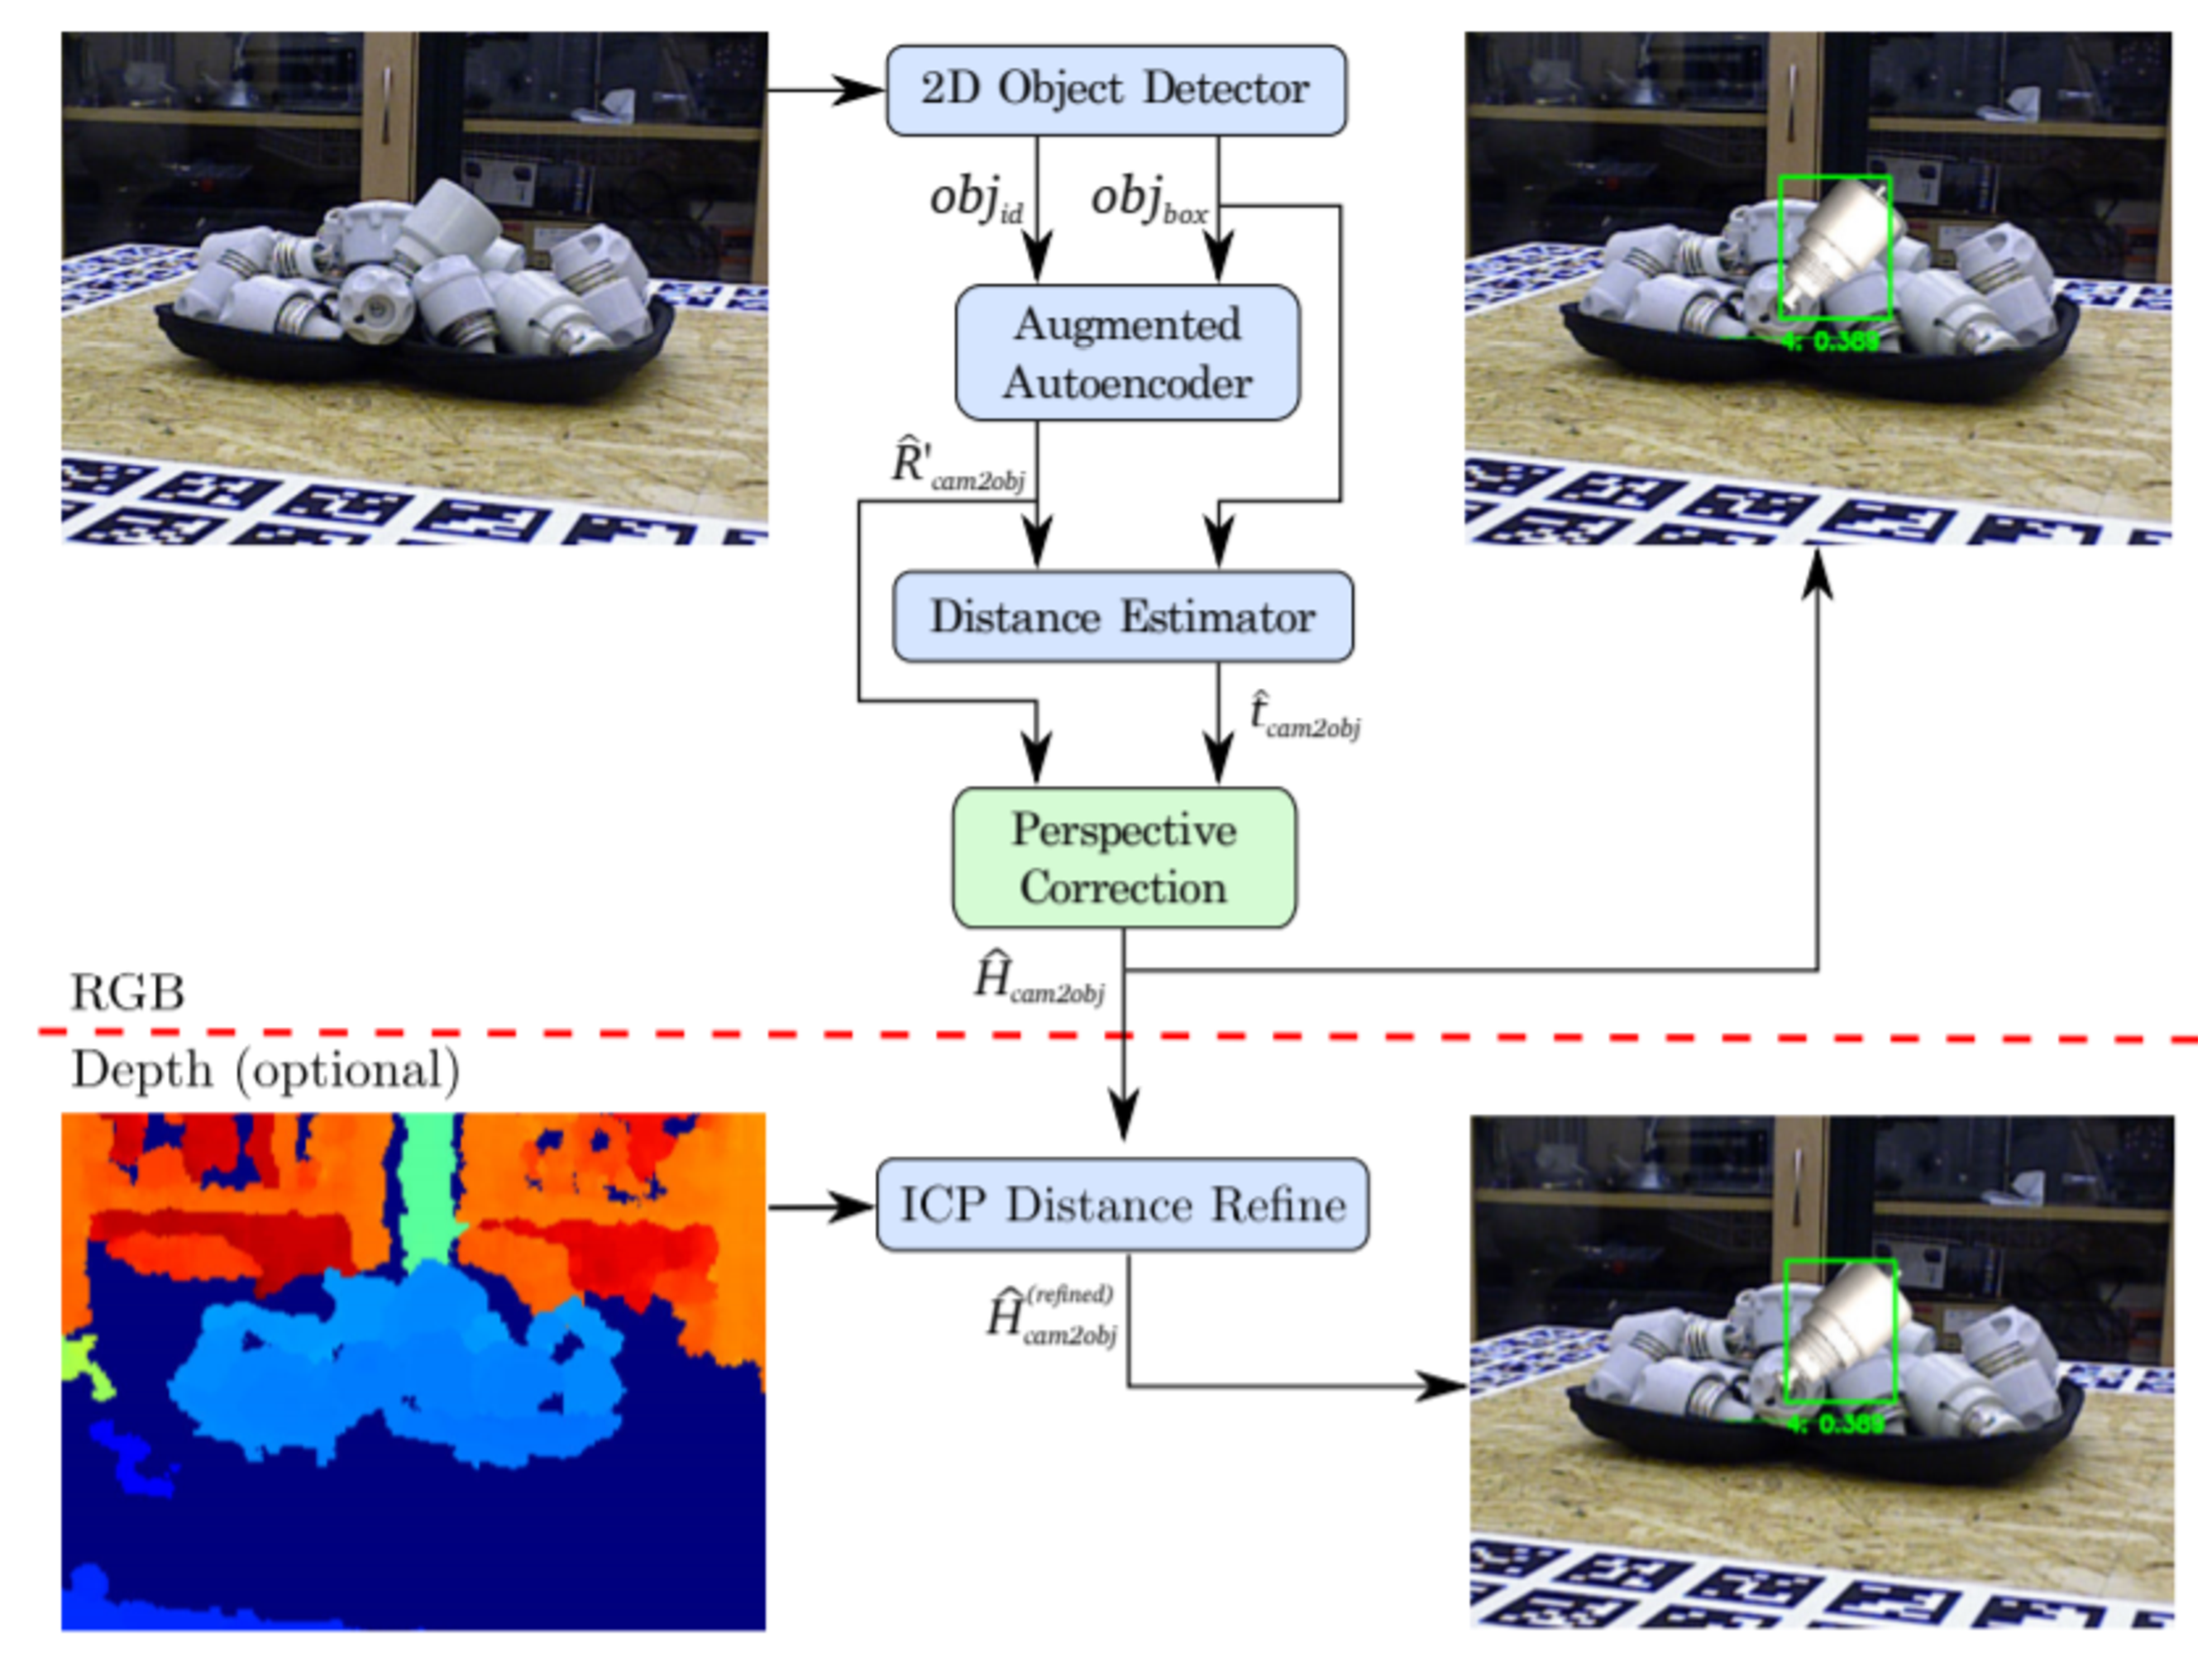
\includegraphics[width=100mm]{figure/eps/6次元推定.eps}
      \caption{6次元物体検出.}
      \label{fig:2d_pose_estimation}
      \end{center}
      \end{figure}



入力となるRGB画像に対してSSD\cite{SSD}を用いて対象物体のID,座標位置,Bounding Boxを検出する.
その後,検出されたBounding Box領域から物体の姿勢情報をAugumented Autoencoderにより取得し,推定を行う.
 


\subsection{Augumented Autoencoder}
AAEの基礎となるのがAutoencoder\cite{AE}である,オートエンコーダーは訓練データのみを使用する教師なし学習の一つである.入力データ$x_i$をエンコーダー$\phi$に入力し,デコーダ$\psi$から得られる出力$x’_i$との損失関数式(\ref{eq:polynomial2})を計算し学習を行い,データを表現する潜在変数zを獲得するためのニューラルネットワークである.潜在変数は式(\ref{eq:polynomial1})によって求められる.

\begin{eqnarray}
\label{eq:polynomial2}
l_2=  \sum_{i}\parallel{ x_i - x'_i} \parallel_2
\end{eqnarray}

\begin{eqnarray}
\label{eq:polynomial1}
( x ^ {\prime})  = (\psi \times  \phi )( x ) = \psi (z)
\end{eqnarray}



AAEでは,オートエンコーダーを発展させたノイズ除去を行い潜在変数を取得するDenoising Autoencoder\cite{DAE}が応用されている.
エンコーダーに訓練データの一部にノイズを加えた画像を入力し,ノイズなしの画像を出力できるよう,
ノイズのない訓練データとの損失関数を学習させることで,
ノイズによらない本質的な潜在表現を得ることができる方法である.

また,Domain Randomization\cite{Dm}という手法も取り入れられている.
この手法の目的は,評価時にモデルが実世界のデータに一般化できるよう,
環境ノイズを加えた3Dモデルをランダムに作成し学習を行う.
これにより物体と背景の対称性を明確にして,評価時に現実世界での推定も可能になる.

上記のDenoising AutoencoderとDomain Randomizationの手法を取り入れ応用したオートエンコーダーがAAEである.
AAEの学習を図\ref{AAEgakusyu}に示す.図\ref{AAEgakusyu}(a)の訓練データxに背景や光,遮蔽物などの環境ノイズ$f_augm$を追加した図\ref{AAEgakusyu}(b)の画像x''を入力し,環境ノイズなしの図\ref{AAEgakusyu}(c)の画像x'を出力するように
xとx"損失関数を計算し学習を行う.データを表現する潜在変数を式(\ref{eq:polynomial3})によって獲得する手法である.

      \begin{figure}[htbp]
      \begin{center}
      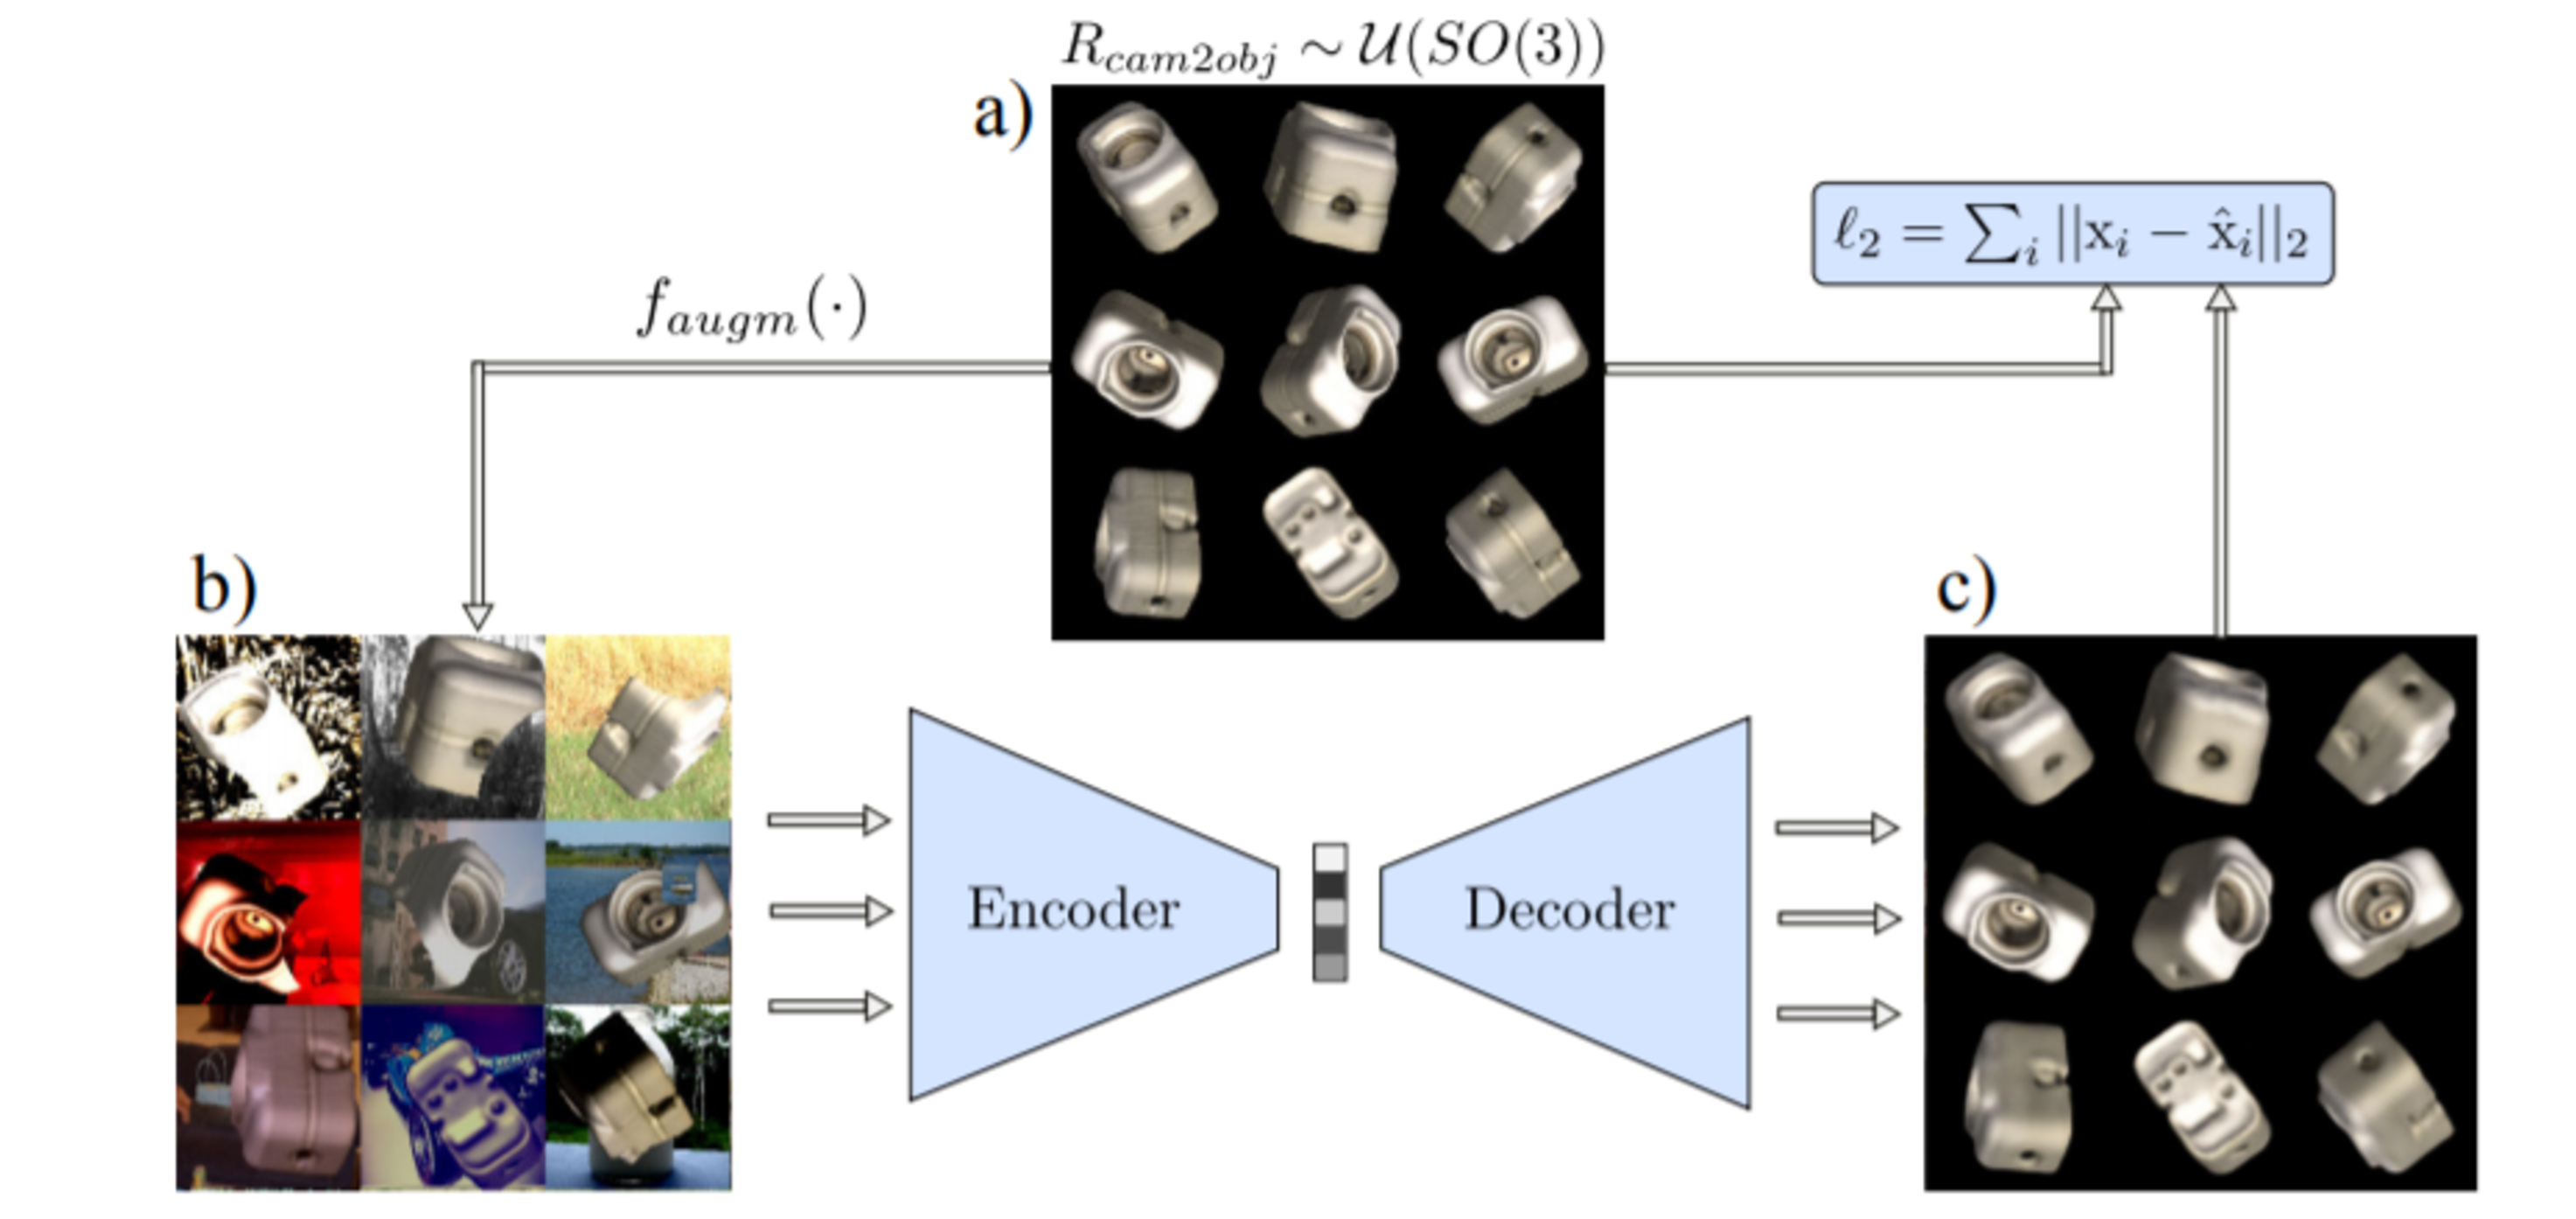
\includegraphics[width=110mm]{figure/eps/AAEの学習.eps}
      \caption{AAEの学習\cite{AAE}.}
      \label{AAEgakusyu}
      \end{center}
      \end{figure}

\begin{eqnarray}
\label{eq:polynomial3}
x ' = (\psi \times  \phi \times f_{augm} )( x ) = (\psi \times \phi) (x'') = \psi (z)
\end{eqnarray}


AAEのネットワークを図\ref{netwa}に示す.入力出力はチャンネル数3の画像サイズ128$\times$128のカラー画像を使用する.

      \begin{figure}[htbp]
      \begin{center}
      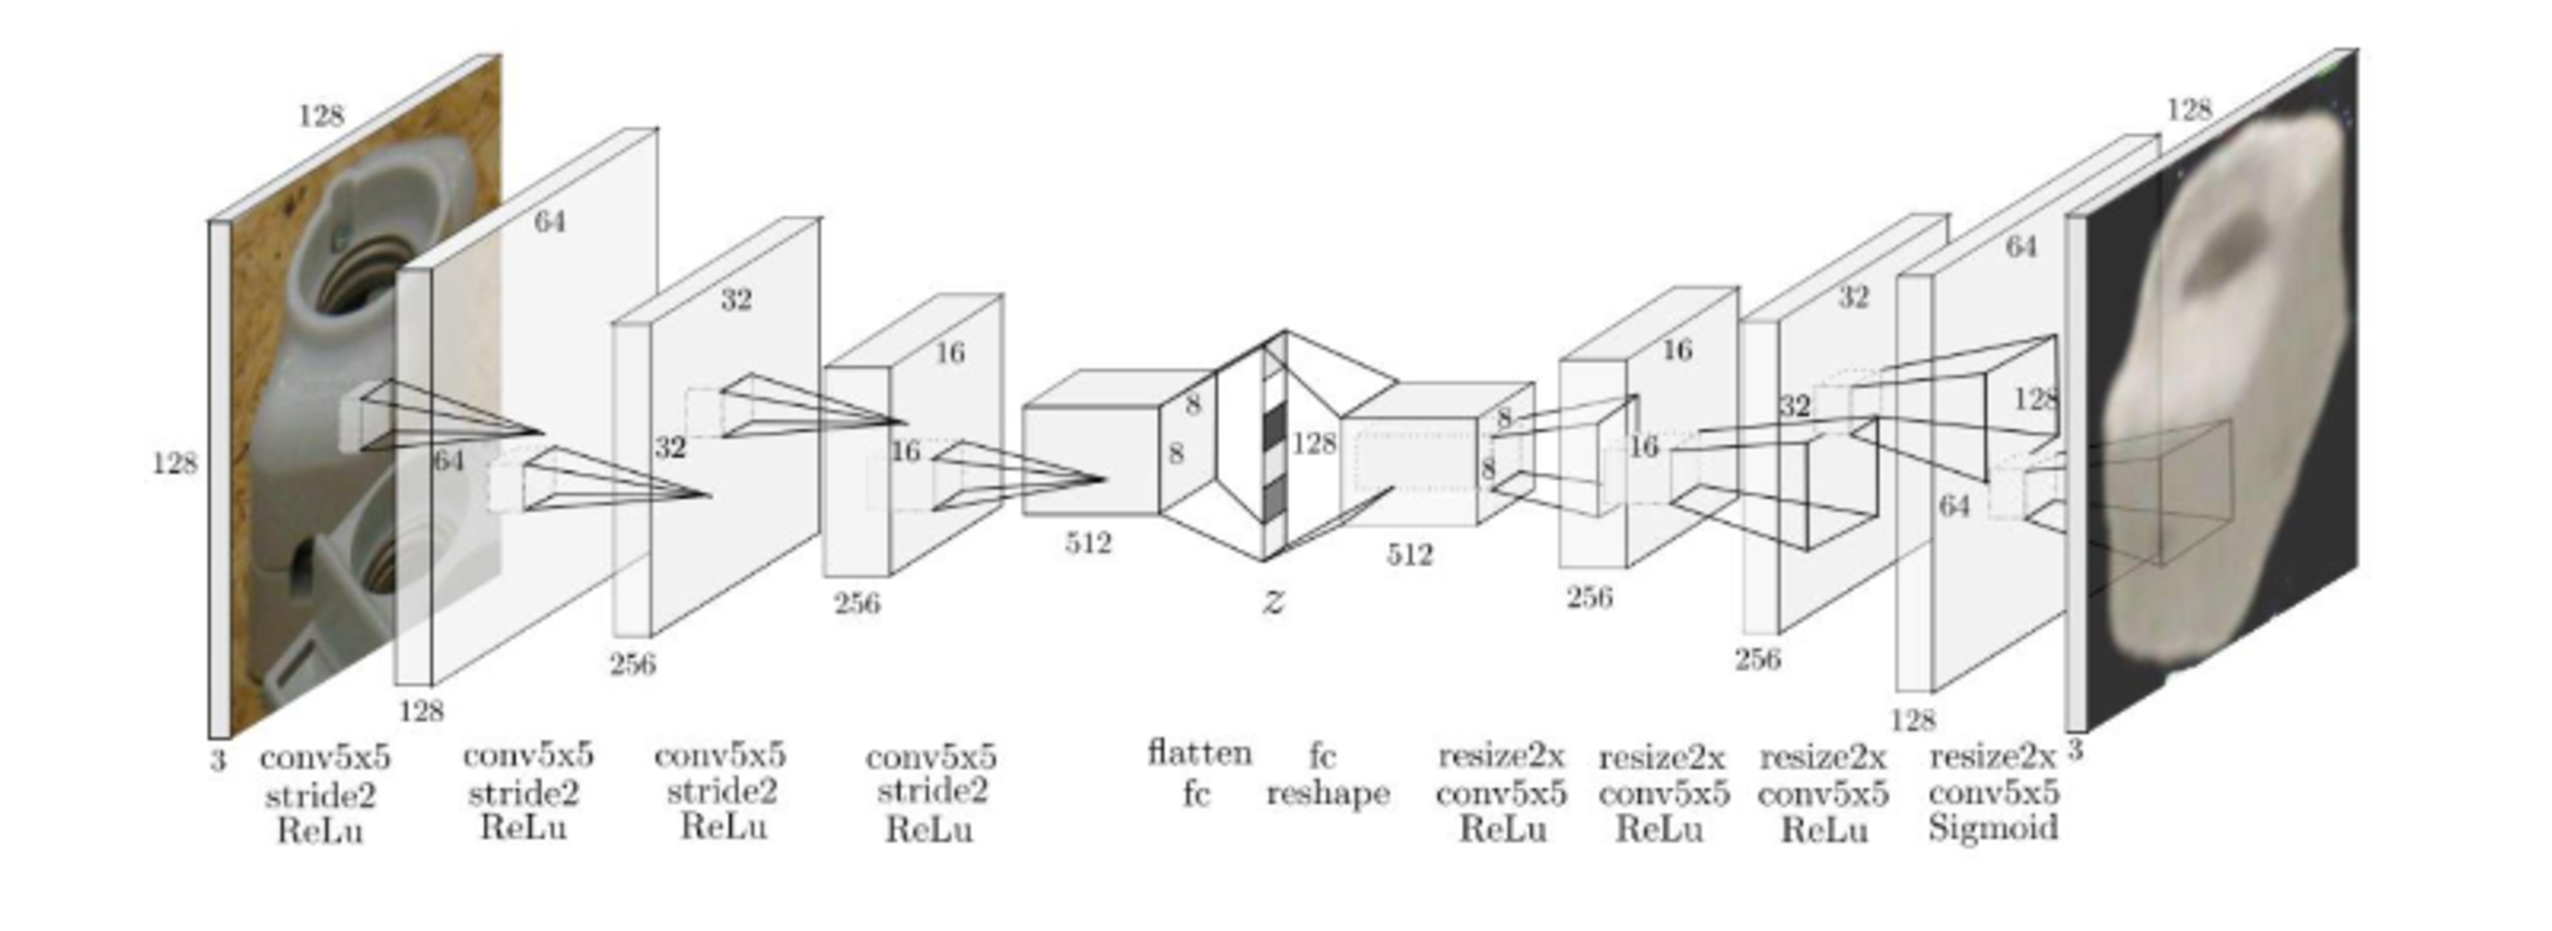
\includegraphics[width=120mm]{figure/eps/ネットワーク.eps}
      \caption{AAEのネットワーク\cite{AAE}.}
      \label{netwa}
      \end{center}
      \end{figure}





\subsection{AAEを用いた姿勢推定}


AAEによって求められる潜在変数を元に姿勢推定を行う.
推定対象となる物体の3Dモデルを作成し,3Dモデル物体を回転させ92232個の姿勢をAAEにかけ潜在変数を生成し92232個分の姿勢情報を持つ潜在変数を記録していく.
記録されている姿勢情報が既知となっている潜在変数$ z_i $と推定したい画像から新たに得た潜在変数$z_{test}$のコサイン類似度を式(\ref{cos})用いて比較し
最も近い潜在変数を持つ姿勢情報を推定姿勢として決定する.

\begin{eqnarray}
\label{cos}
cos_i = \frac {z_i \times z_{test}}{|z_i||z_{test}|}
\end{eqnarray}


%----------------------------------------------


%----------------------------------------------
\chapter{提案手法}
\label{chap:3}
本章では,提案手法について示す.

\section{変形ARマーカの姿勢推定}
提案手法は,円柱に貼り変形したARマーカを機械学習を用いて平面状のARマーカへの復元を行い,
復元を行うときにエンコードされる潜在変数を用いて姿勢推定を行う.
提案手法では,訓練データを円柱に貼られた変形ARマーカに背景テクスチャをつけた図\ref{hennkei}に示す
画像のように用意する.

      \begin{figure}[htbp]
      \begin{center}
      
\includegraphics[width=50mm]{figure/eps/変形.eps}
      \caption{訓練データ.}
      \label{hennkei}
      \end{center}
      \end{figure}

訓練データと同じ姿勢の円柱に貼り付けられた平面状のARマーカ図\ref{heimen}に示す画像のように教師データ
を用意する.提案手法は教師データを使用する教師あり学習を行うオートエンコーダーを用いて
,平面状のARマーカへの復元を行う.

      \begin{figure}[htbp]
      \begin{center}
      
\includegraphics[width=50mm]{figure/eps/平面.eps}
      \caption{教師データ.}
      \label{heimen}
      \end{center}
      \end{figure}

\subsection{学習}
提案手法のオートエンコーダーの学習の流れを図\ref{gakusyu}に示す.
訓練データ図\ref{gakusyu}(b)をオートエンコーダに入力し,出力図\ref{gakusyu}(c)と教師データ図\ref{gakusyu}(a)の損失関数を計算し
差分が小さくなるように学習を行っていく.学習を行うことで変形ARマーカの姿勢を
表現する潜在変数を獲得することができる.
      \begin{figure}[htbp]
      \begin{center}
      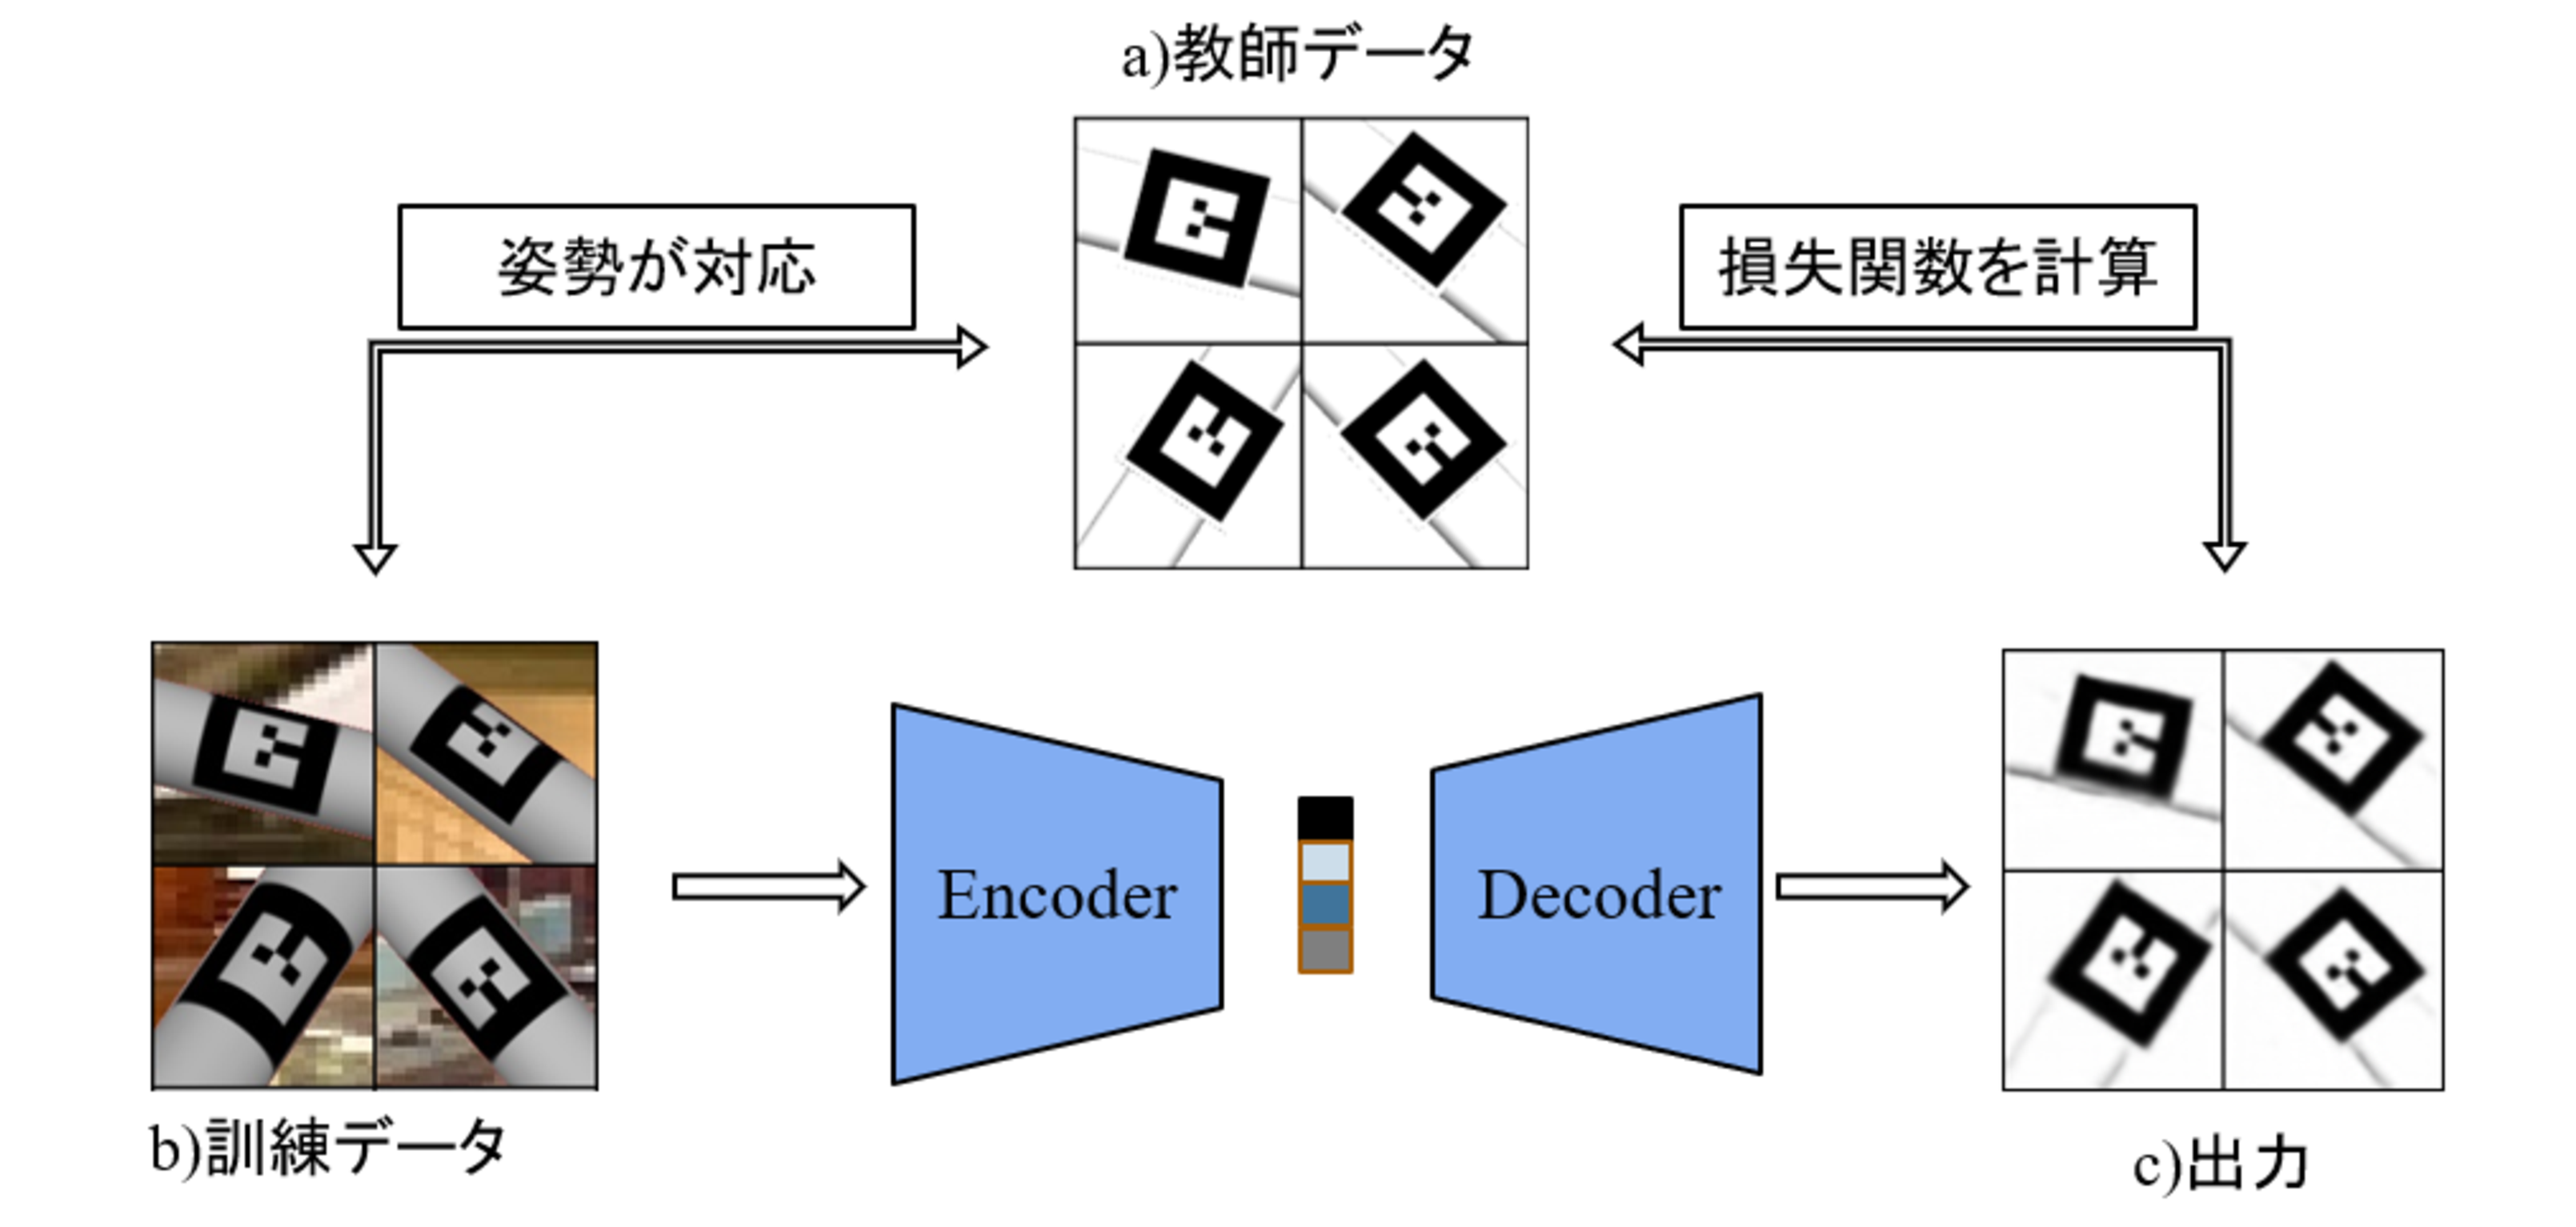
\includegraphics[width=100mm]{figure/eps/提案手法の学習.eps}
      \caption{提案手法の学習の流れ.}
      \label{gakusyu}
      \end{center}
      \end{figure}


\subsection{提案手法による姿勢推定}
姿勢推定を行うためにはデータベースを作成しておく必要がある.データベース作成の流れを図\ref{データベース}に示す.
データベースは,ARマーカの姿勢をrollを0$\sim$360度, pitchを-35$\sim$35度, yawを-15$\sim$15度に範囲を設定し,角度3度刻みで回転させた分解能3度で姿勢画像36,000枚を用意し,エンコーダーに入力する.出力された36,000枚分の潜在変数$z_n$をデータベースとして用意する.

      \begin{figure}[htbp]
      \begin{center}
      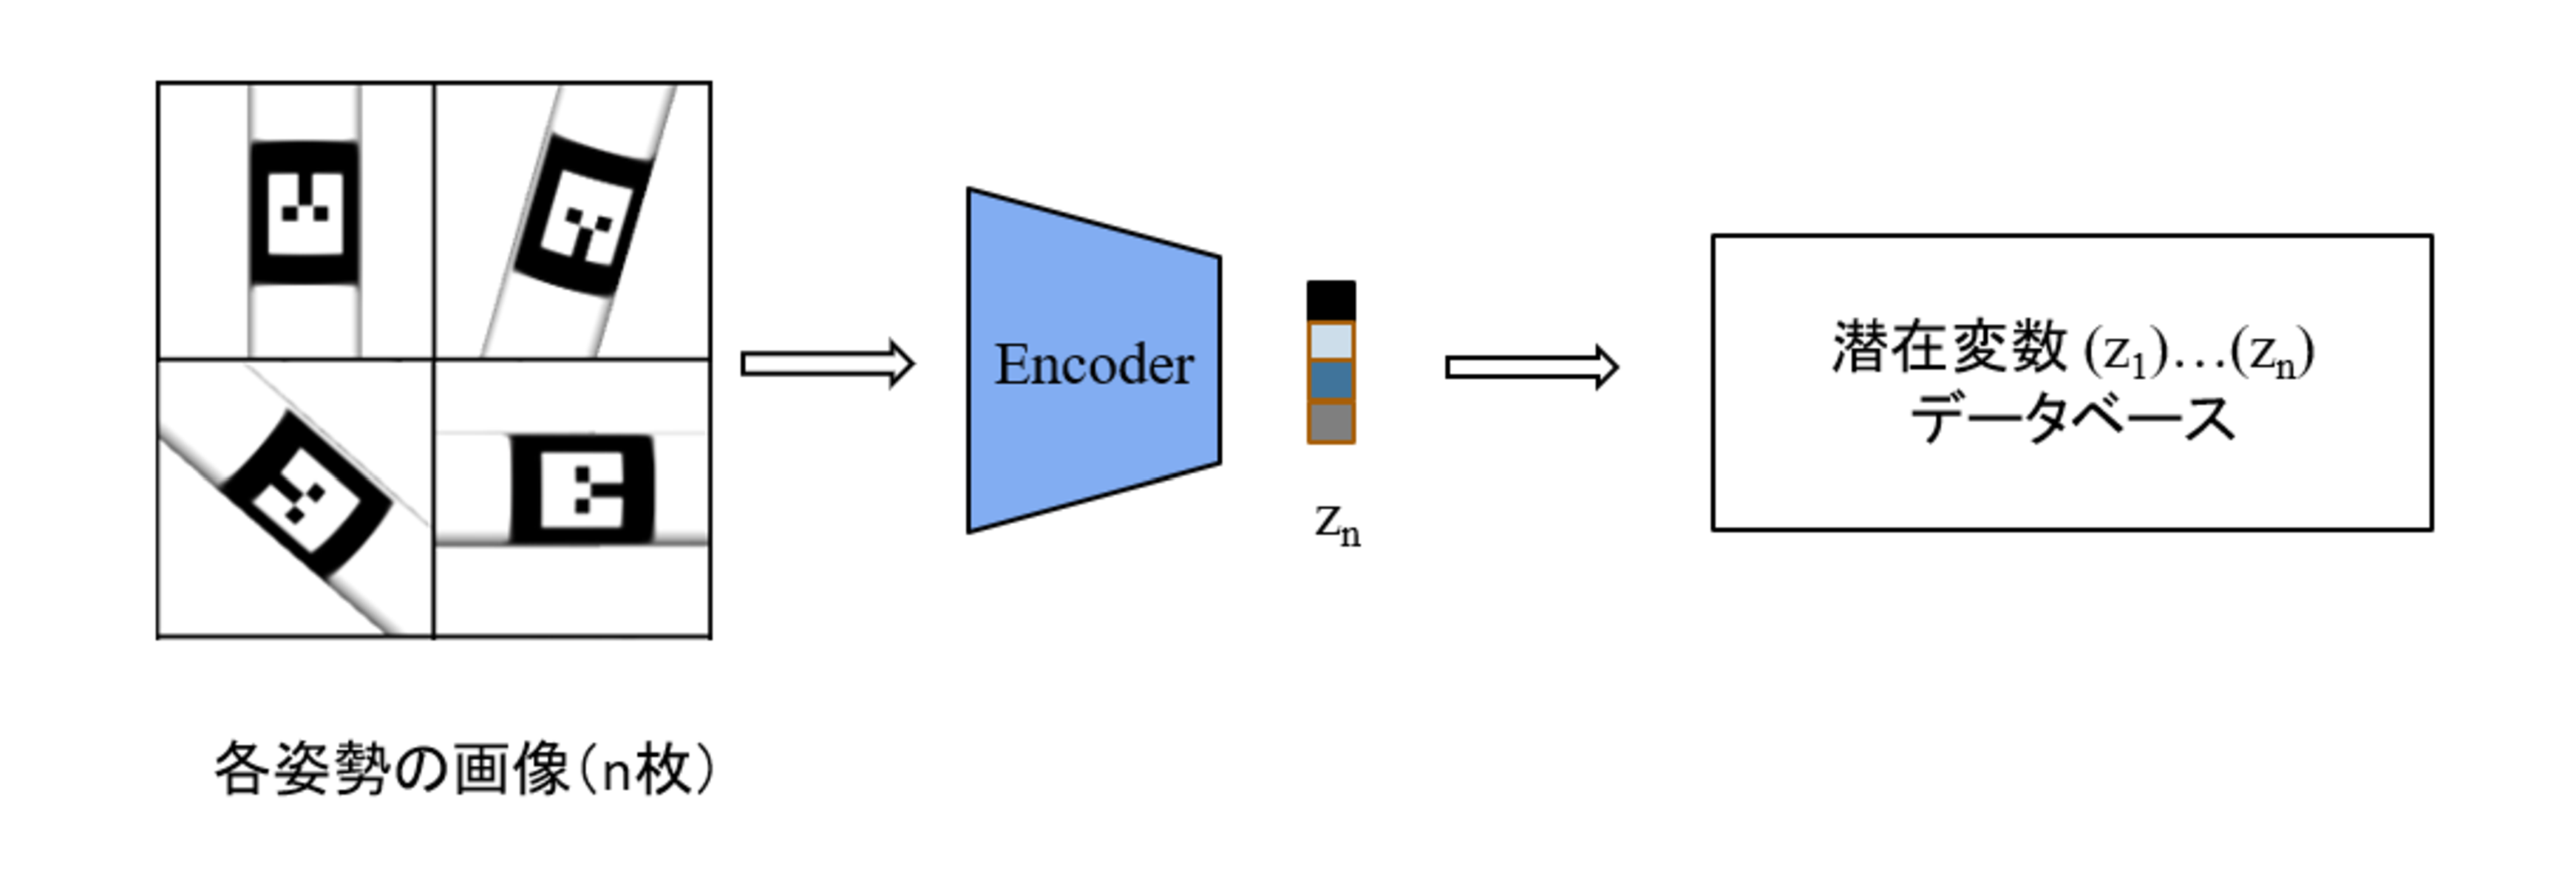
\includegraphics[width=100mm]{figure/eps/データベース.eps}
      \caption{データベースの作成.}
      \label{データベース}
      \end{center}
      \end{figure}

提案手法で行う姿勢推定の流れを図\ref{suitei}に示す.推定対象となる画像を学習済みのオートエンコーダーに入力し潜在変数を取得する.その後,各姿勢の潜在変数を保存したデータベースとの潜在変数をコサイン類似度を用いて最も近い値のデータベースの姿勢を推定姿勢として決定する.

      \begin{figure}[htbp]
      \begin{center}
      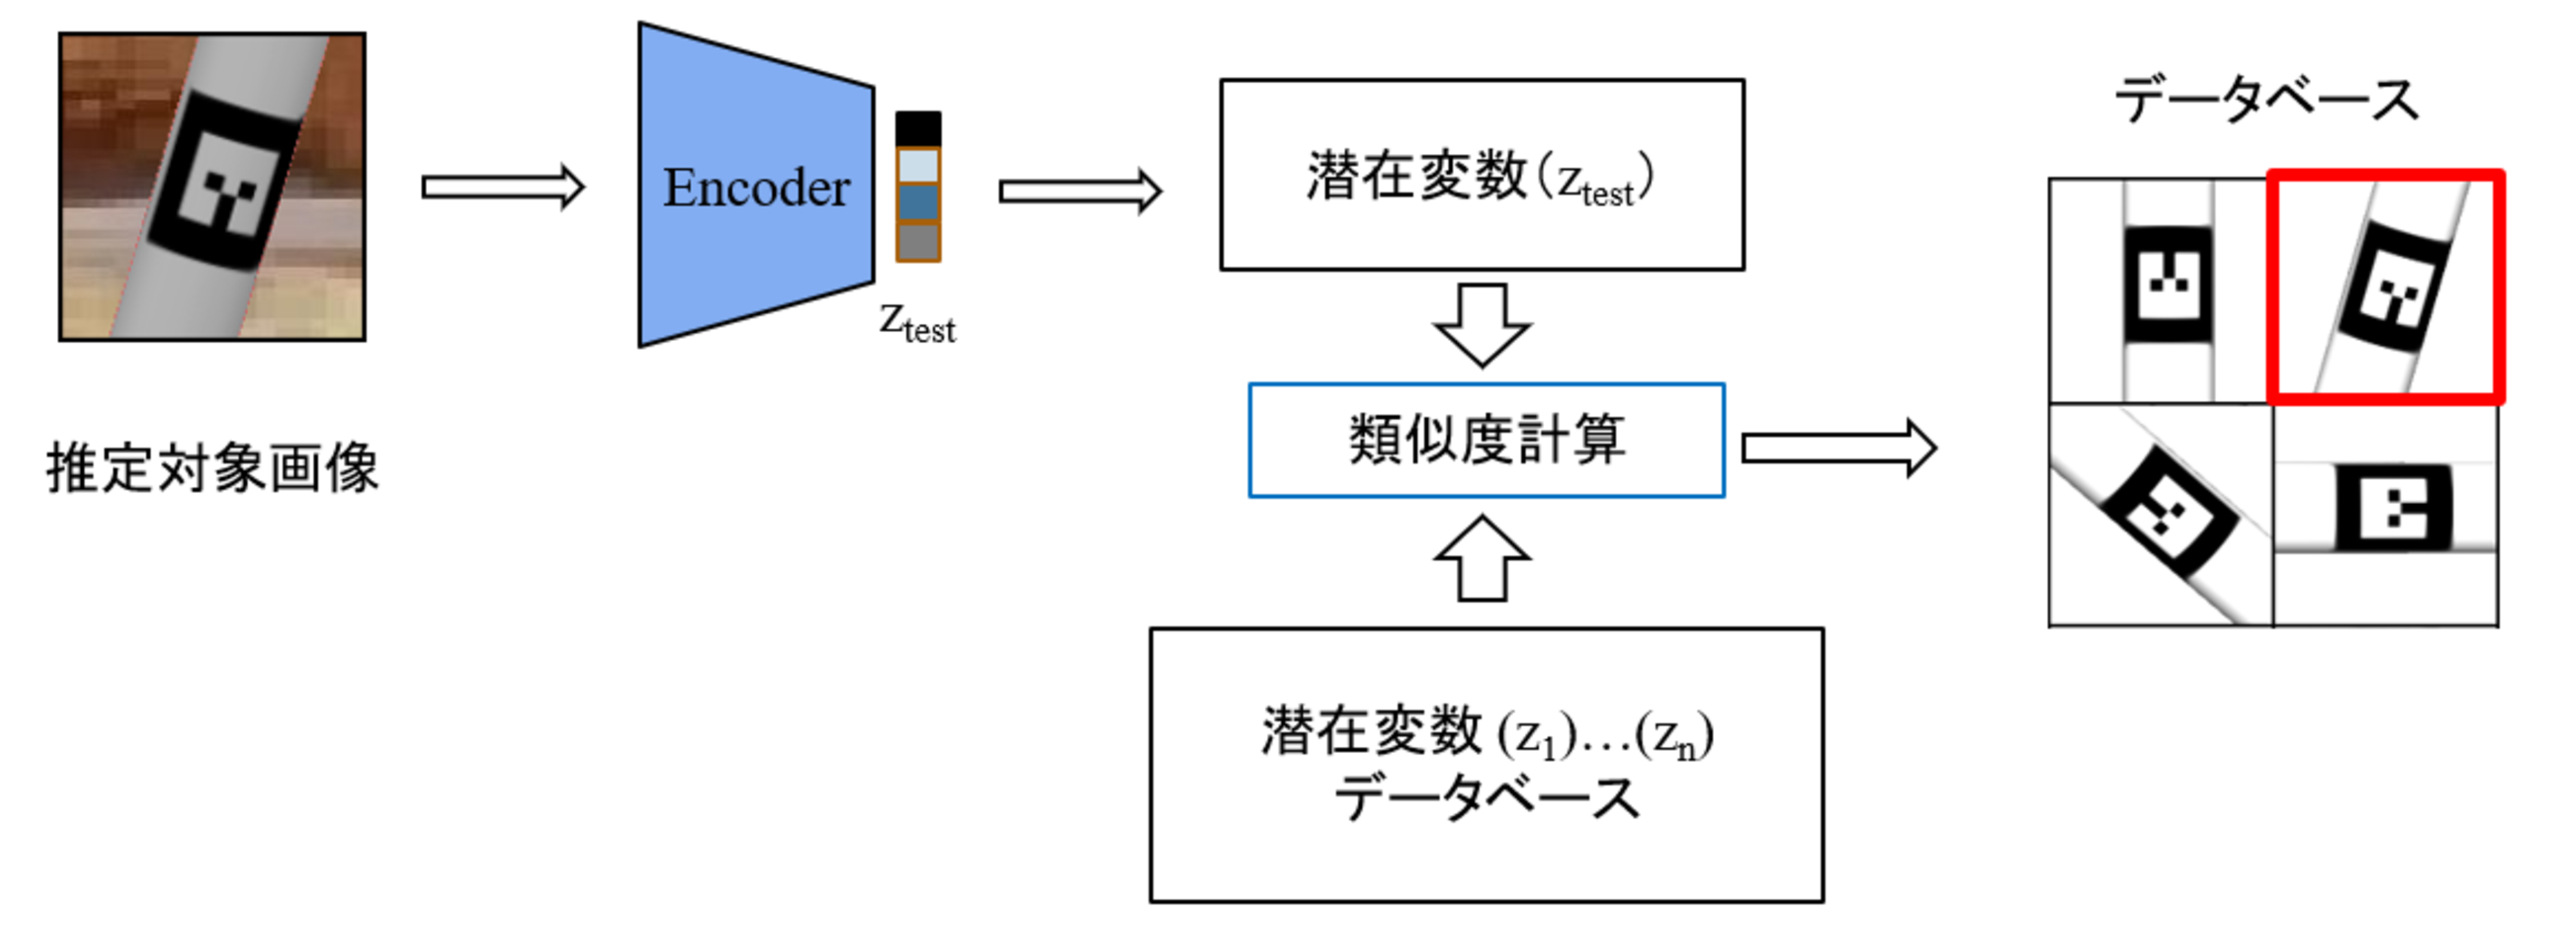
\includegraphics[width=100mm]{figure/eps/提案手法の流れ.eps}
      \caption{提案手法による推定.}
      \label{suitei}
      \end{center}
      \end{figure}

\section{学習データの作成}

提案手法では円柱に沿うように貼られた変形ARマーカモデルと円柱に貼られた平面状のARマーカ図\ref{gazebo2}に示す2つのモデルを使用し学習データを用意する.

      \begin{figure}[htbp]
      \begin{center}
      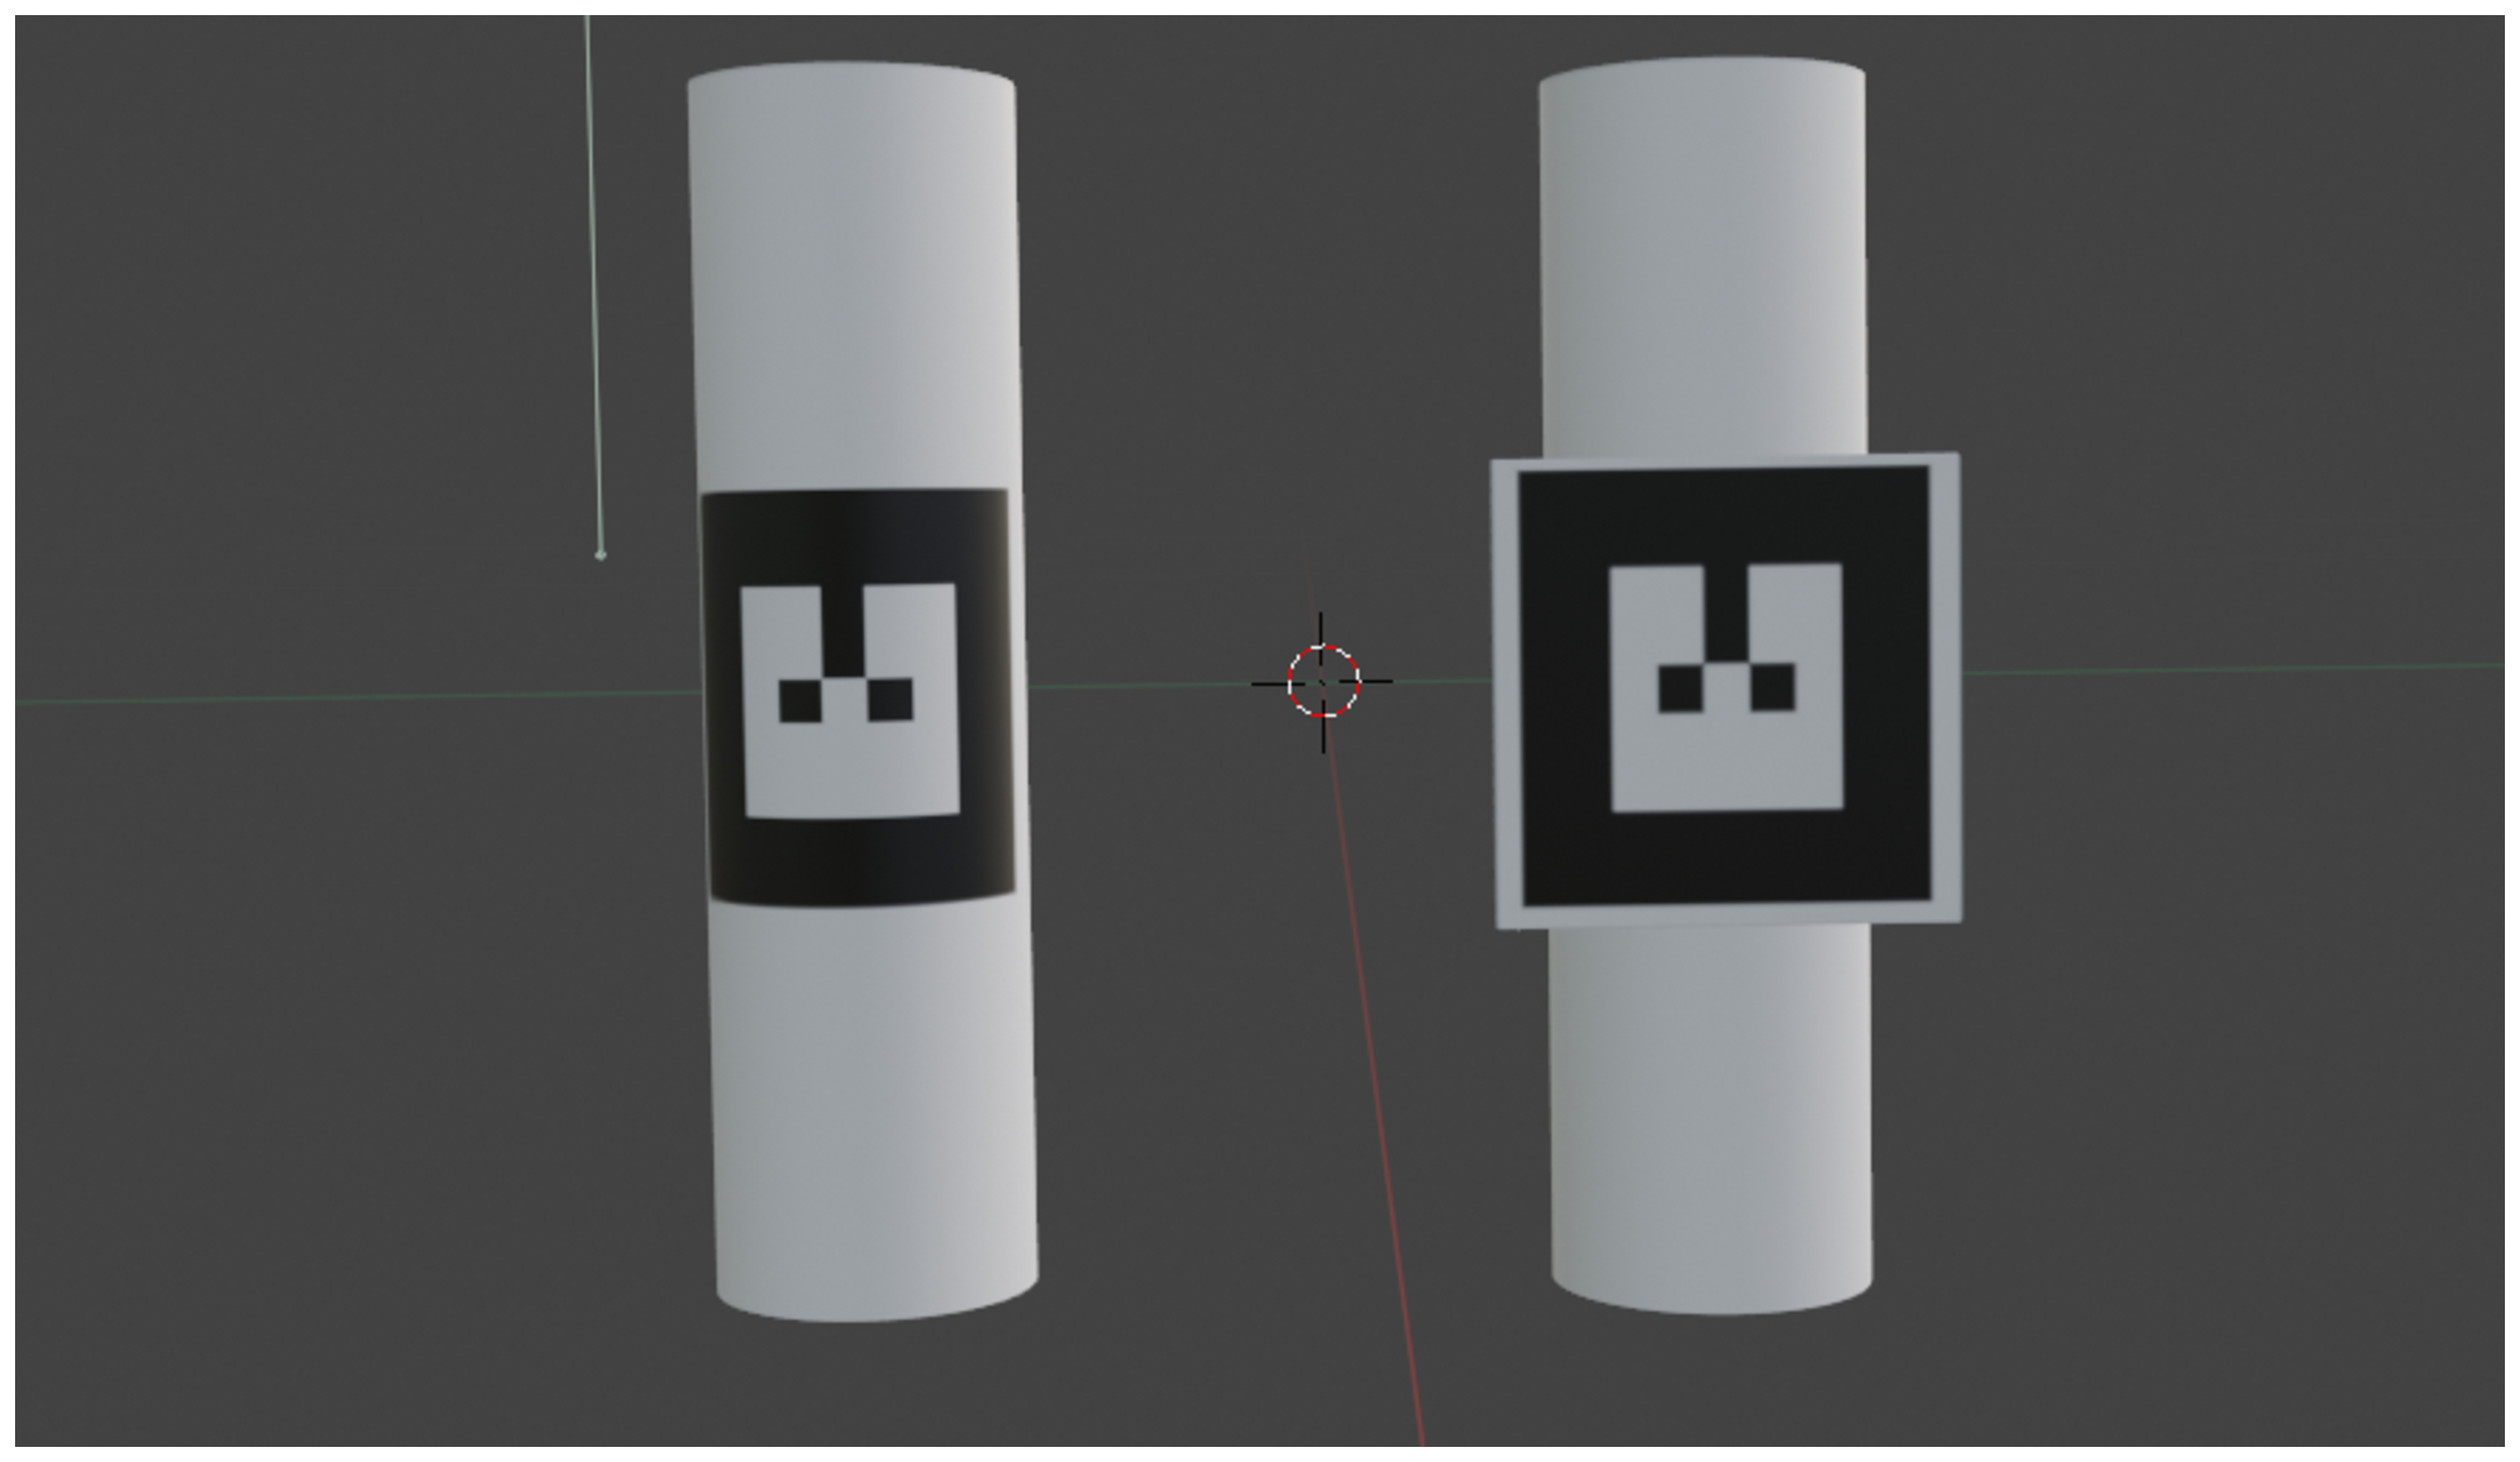
\includegraphics[width=80mm]{figure/eps/二つのモデル.eps}
      \caption{使用するマーカモデル.}
      \label{gazebo2}
      \end{center}
      \end{figure}

\subsection{ARマーカの作成}
ARマーカはROSのパッケージである
ar\_tlack\_alvar
にて用意されている,
マーカID0~9のものを使用する.マーカID0~9を図\ref{09}に示す.

      \begin{figure}[htbp]
      \begin{center}
      \includegraphics[width=80mm]{figure/eps/ARマーカ0~9.eps}
      \caption{使用するARマーカ.}
      \label{09}
      \end{center}
      \end{figure}

ARマーカの大きさはそれぞれ50mmの大きさとなるようにする.
illustratorを用いて変形ARマーカ,平面状ARマーカを円柱モデルに貼り付ける画像を用意する.
平面状のARマーカはblendarを用いて作成する際に50mmの板にARマーカを貼り付け円柱とつなぎ合わせる.
変形ARマーカは直接円柱に貼り付けるため,画素値(255,255,255)の大きさ,縦幅横幅それぞれ作成したい円柱の縦幅と円周に合わせた背景画像にAR マーカが左端中央となるよう貼り画像を作成する.円柱の半径と横幅を表\ref{tab:ARsize}に示す.
\newpage

\begin{table}[h]
  \centering
  \caption{作成するARマーカ画像の大きさ}
    \begin{tabular}{c|c|c} \hline
		半径(mm) & 縦幅(mm) &横幅(mm) \\ \hline \hline
    	20 & 150 & 125.664 \\ \hline
    	30 & 150 & 188.496 \\ \hline
    	40 & 150 & 251.327 \\ \hline
  \end{tabular}
 \label{tab:ARsize}
\end{table}


\subsection{変形ARマーカモデル}

ARマーカを貼り付けた円柱モデルは,blendar\cite{bl}で作成を行う.version2.8を使用する.
blender\cite{bl}を開くと初期状態では立方体が表示されているため削除をする.
図\ref{bl1}に示すように,画面左上の「追加」からメッシュ,cylinderの順番で選択をすると円柱が表示される.


      \begin{figure}[htbp]
      \begin{center}
      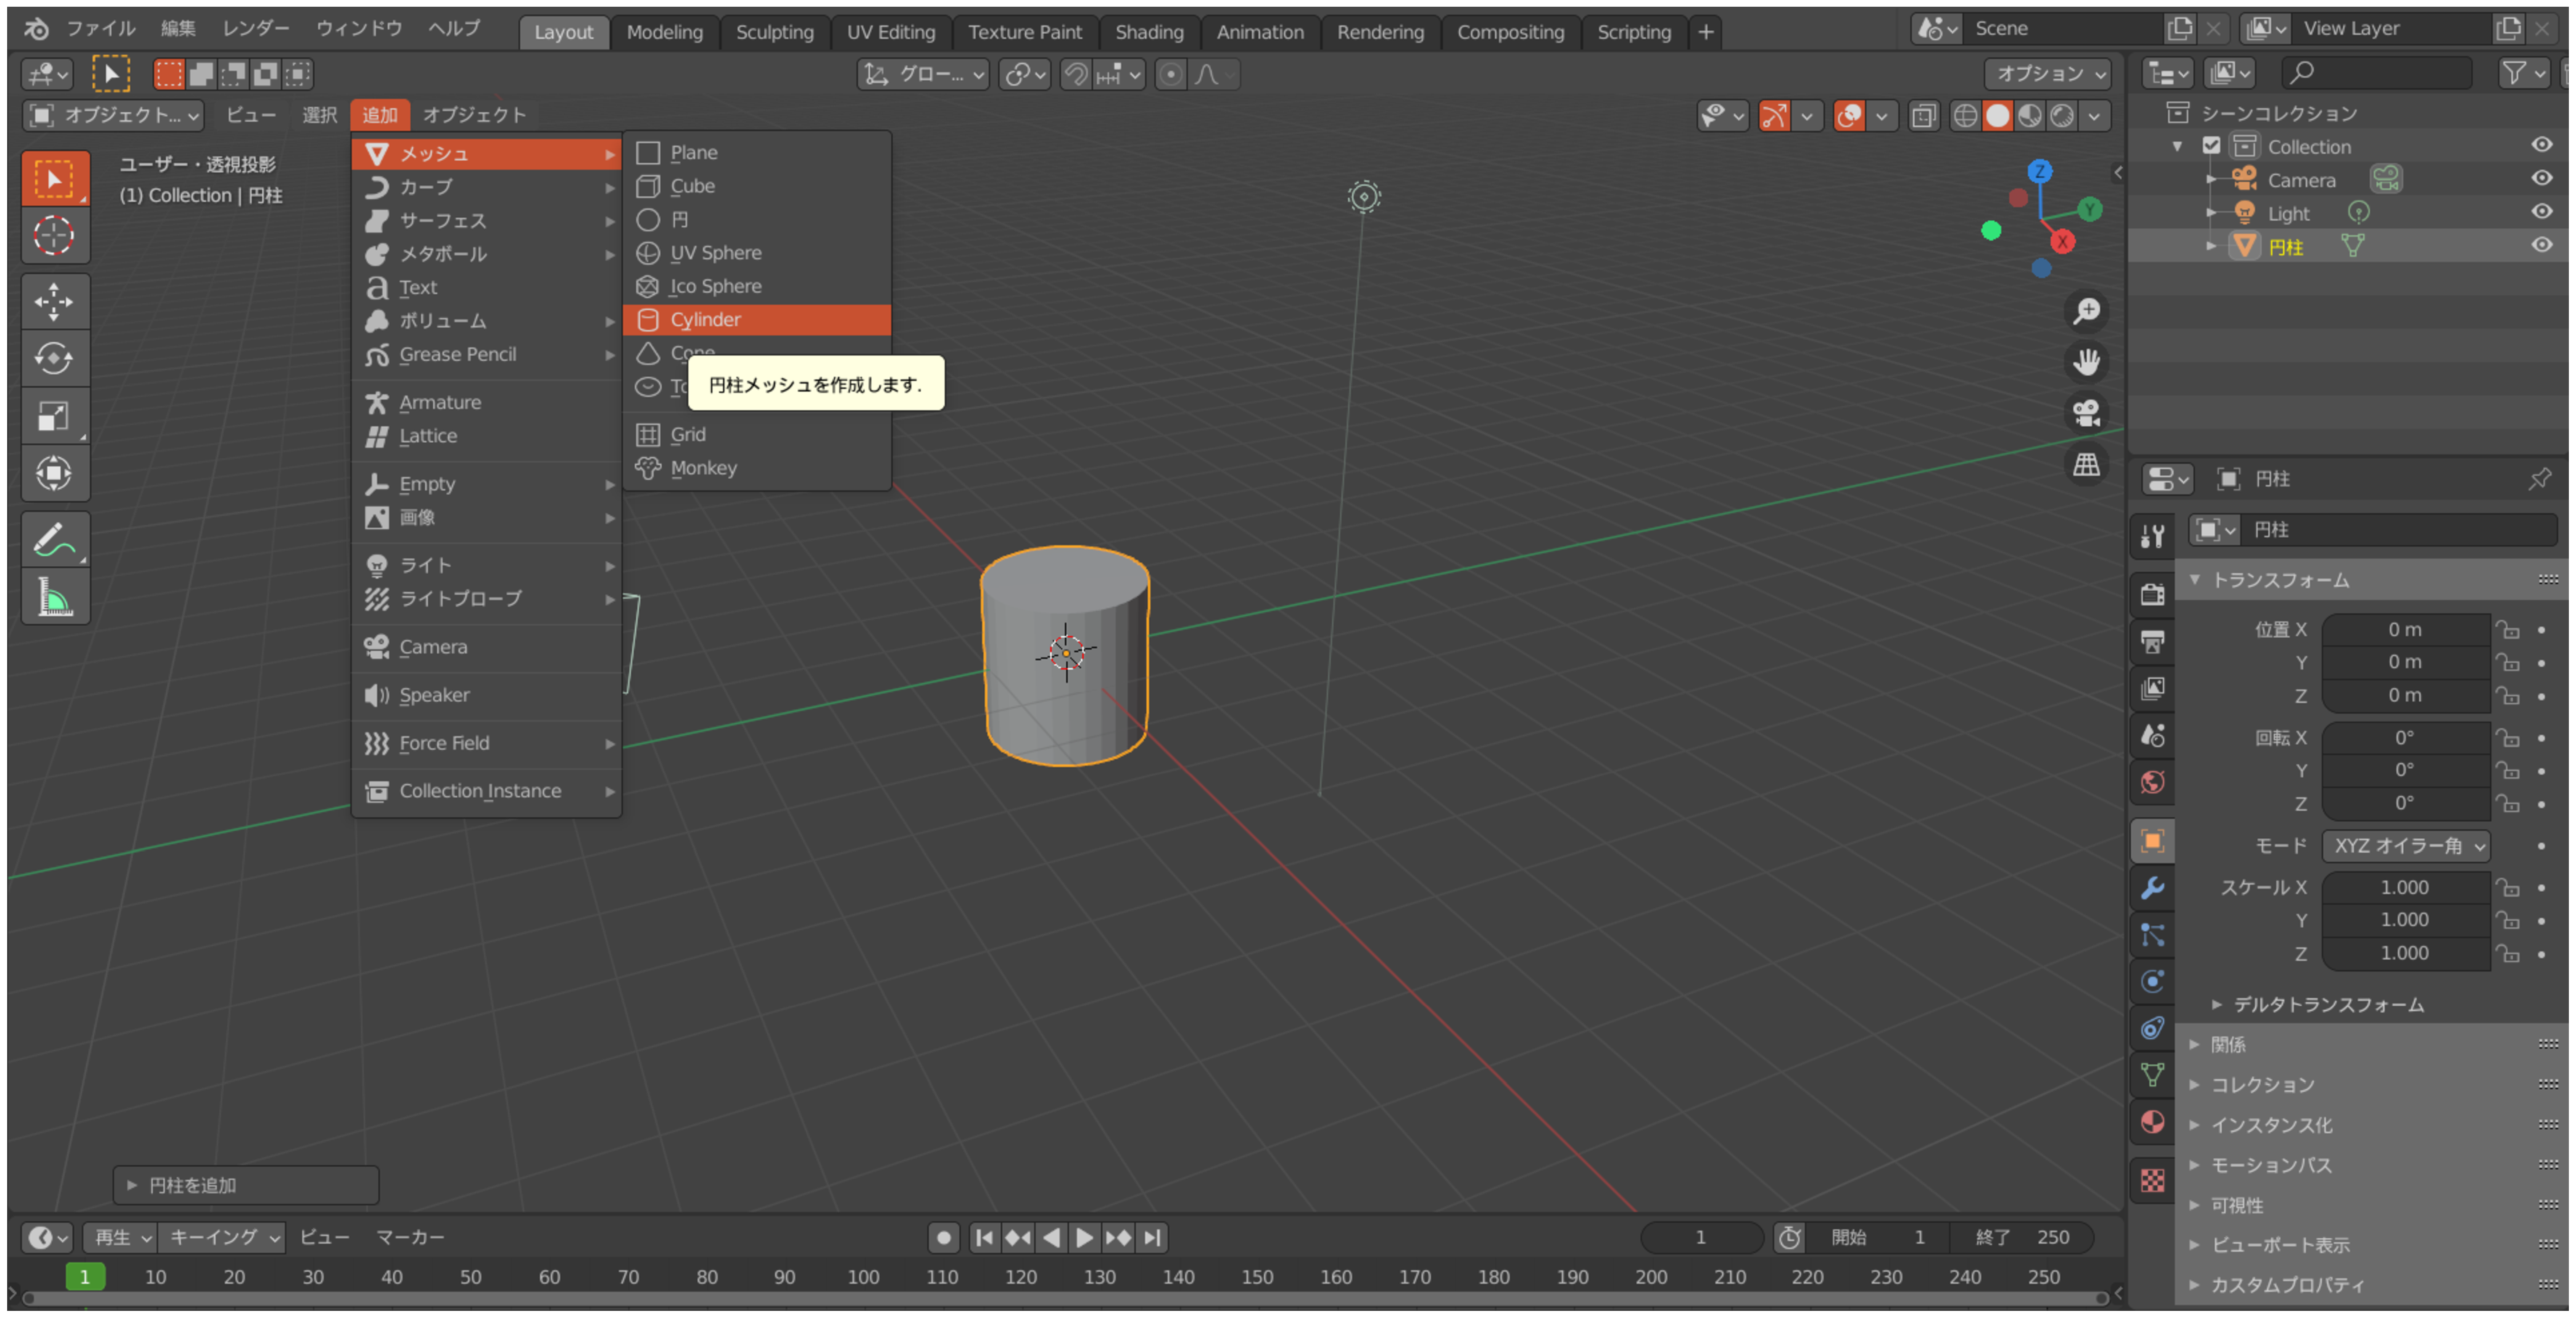
\includegraphics[width=90mm]{figure/eps/bl1.eps}
      \caption{blenderを用いた円柱作成.}
      \label{bl1}
      \end{center}
      \end{figure}




図\ref{bl2}に示すように,左下に表示される「円柱の追加」を選択し,円柱の頂点,半径,深度を変更を行う.
円柱の底面図形は円ではなく正多角形で表現されているため,頂点の数を増やすことで
円に近づける.深度で円柱の縦幅を変えられるため,0.15mに設定する.半径は0.02,0.03,0.04mで用意する.

      \begin{figure}[htbp]
      \begin{center}
      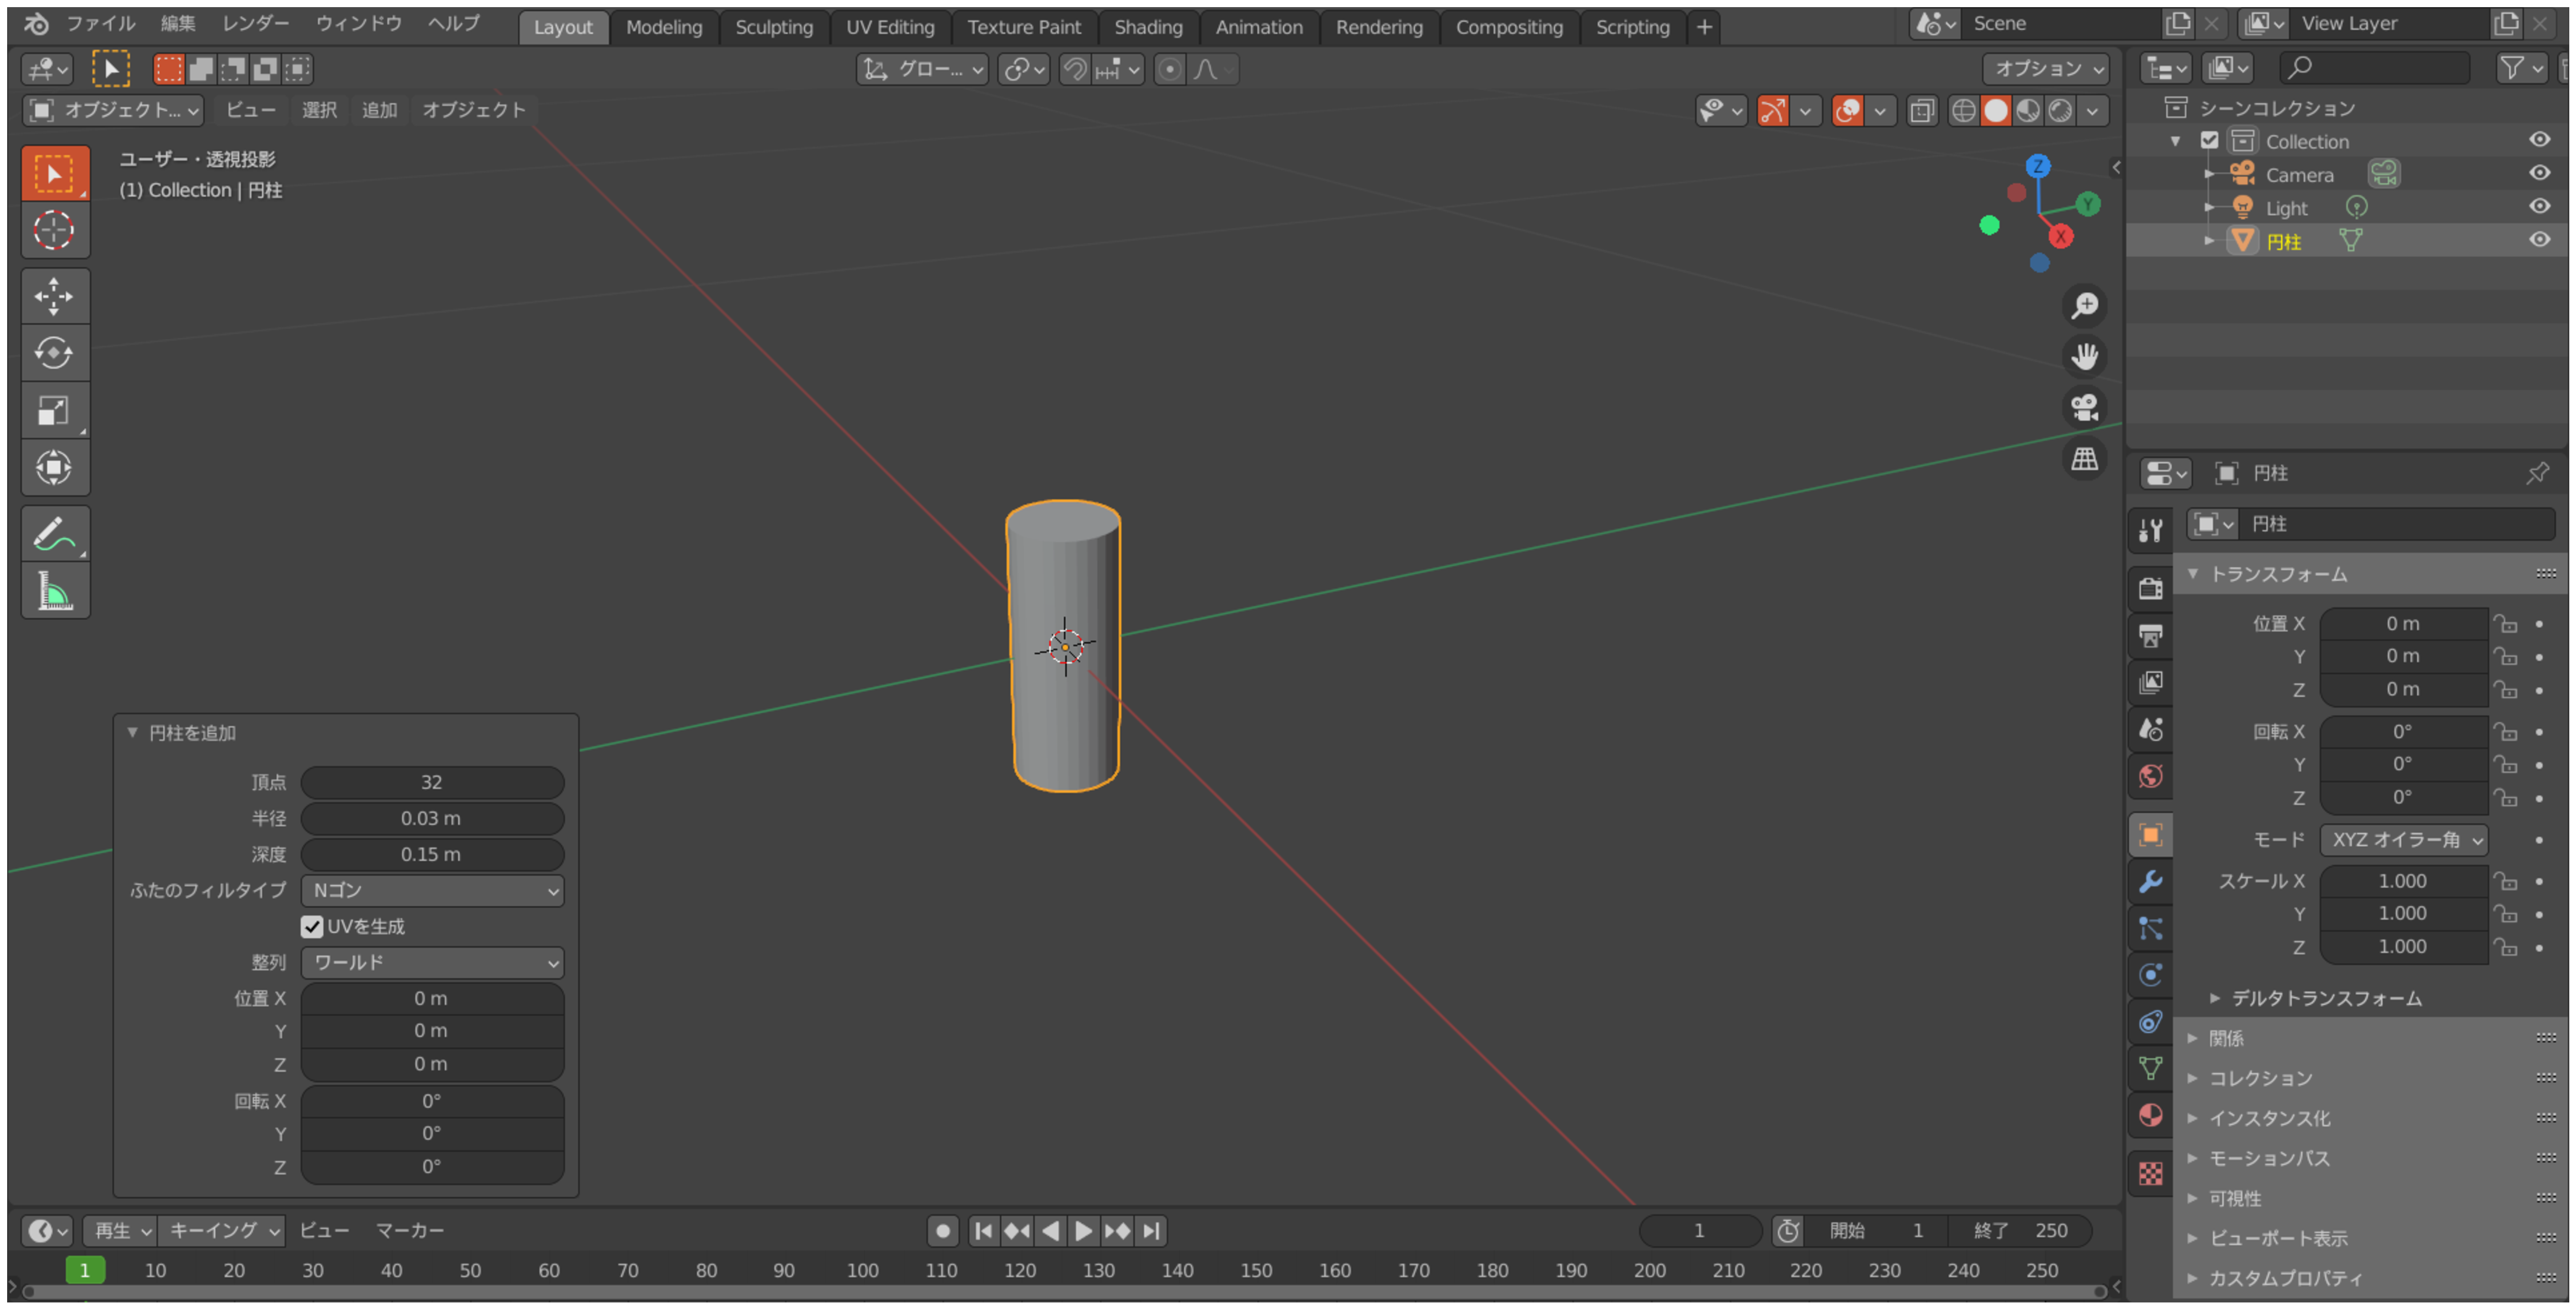
\includegraphics[width=90mm]{figure/eps/bl2.eps}
      \caption{円柱の設定.}
      \label{bl2}
      \end{center}
      \end{figure}

\newpage

画面上部にある「UV Editing」を選択すると画面右側に円柱,左側にマス目が表示される.
編集モードに変更し「面選択」を選択し図\ref{bl3}に示すように底面の削除を行う.

      \begin{figure}[htbp]
      \begin{center}
      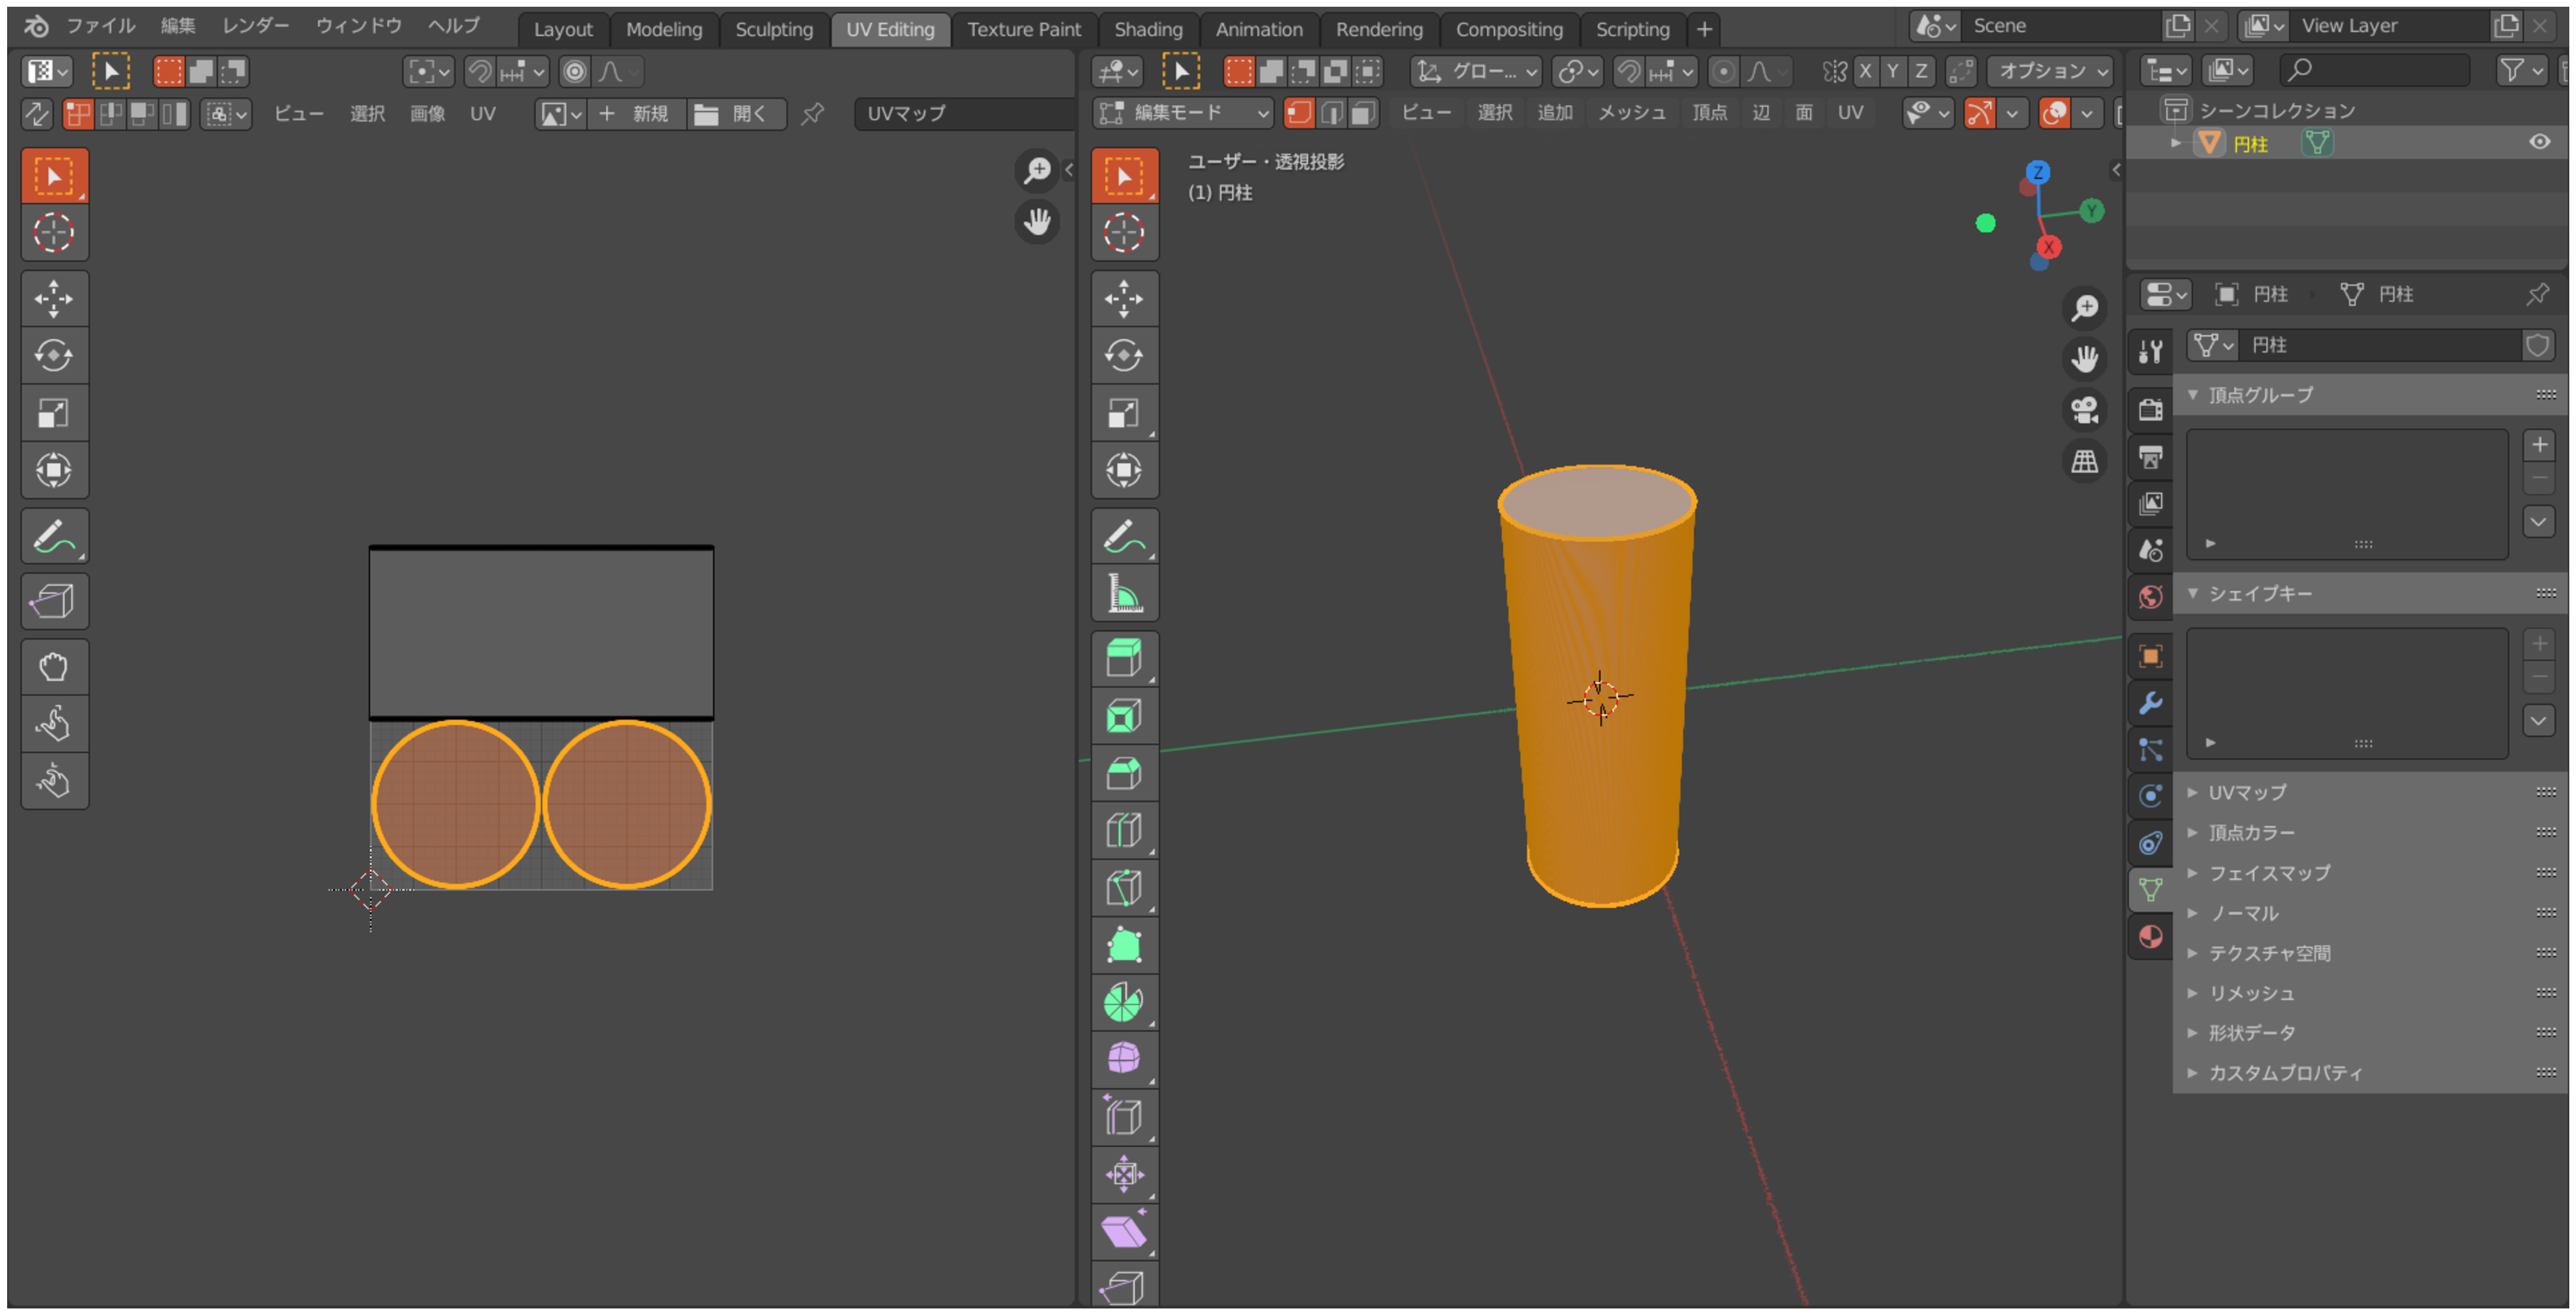
\includegraphics[width=90mm]{figure/eps/bl3.eps}
      \caption{円柱の底面の削除.}
      \label{bl3}
      \end{center}
      \end{figure}




「Modeling」を選択し,画面右下の「Material」を選
択し新規作成を選択,ベースカラーを画像テクスチャにしてから先ほど作成したARマーカ
の画像を開く.右上にあるマテリアルのマークを選択すると図\ref{bl4} のようにAR マーカが貼付
された円柱のモデルができる.


      \begin{figure}[htbp]
      \begin{center}
      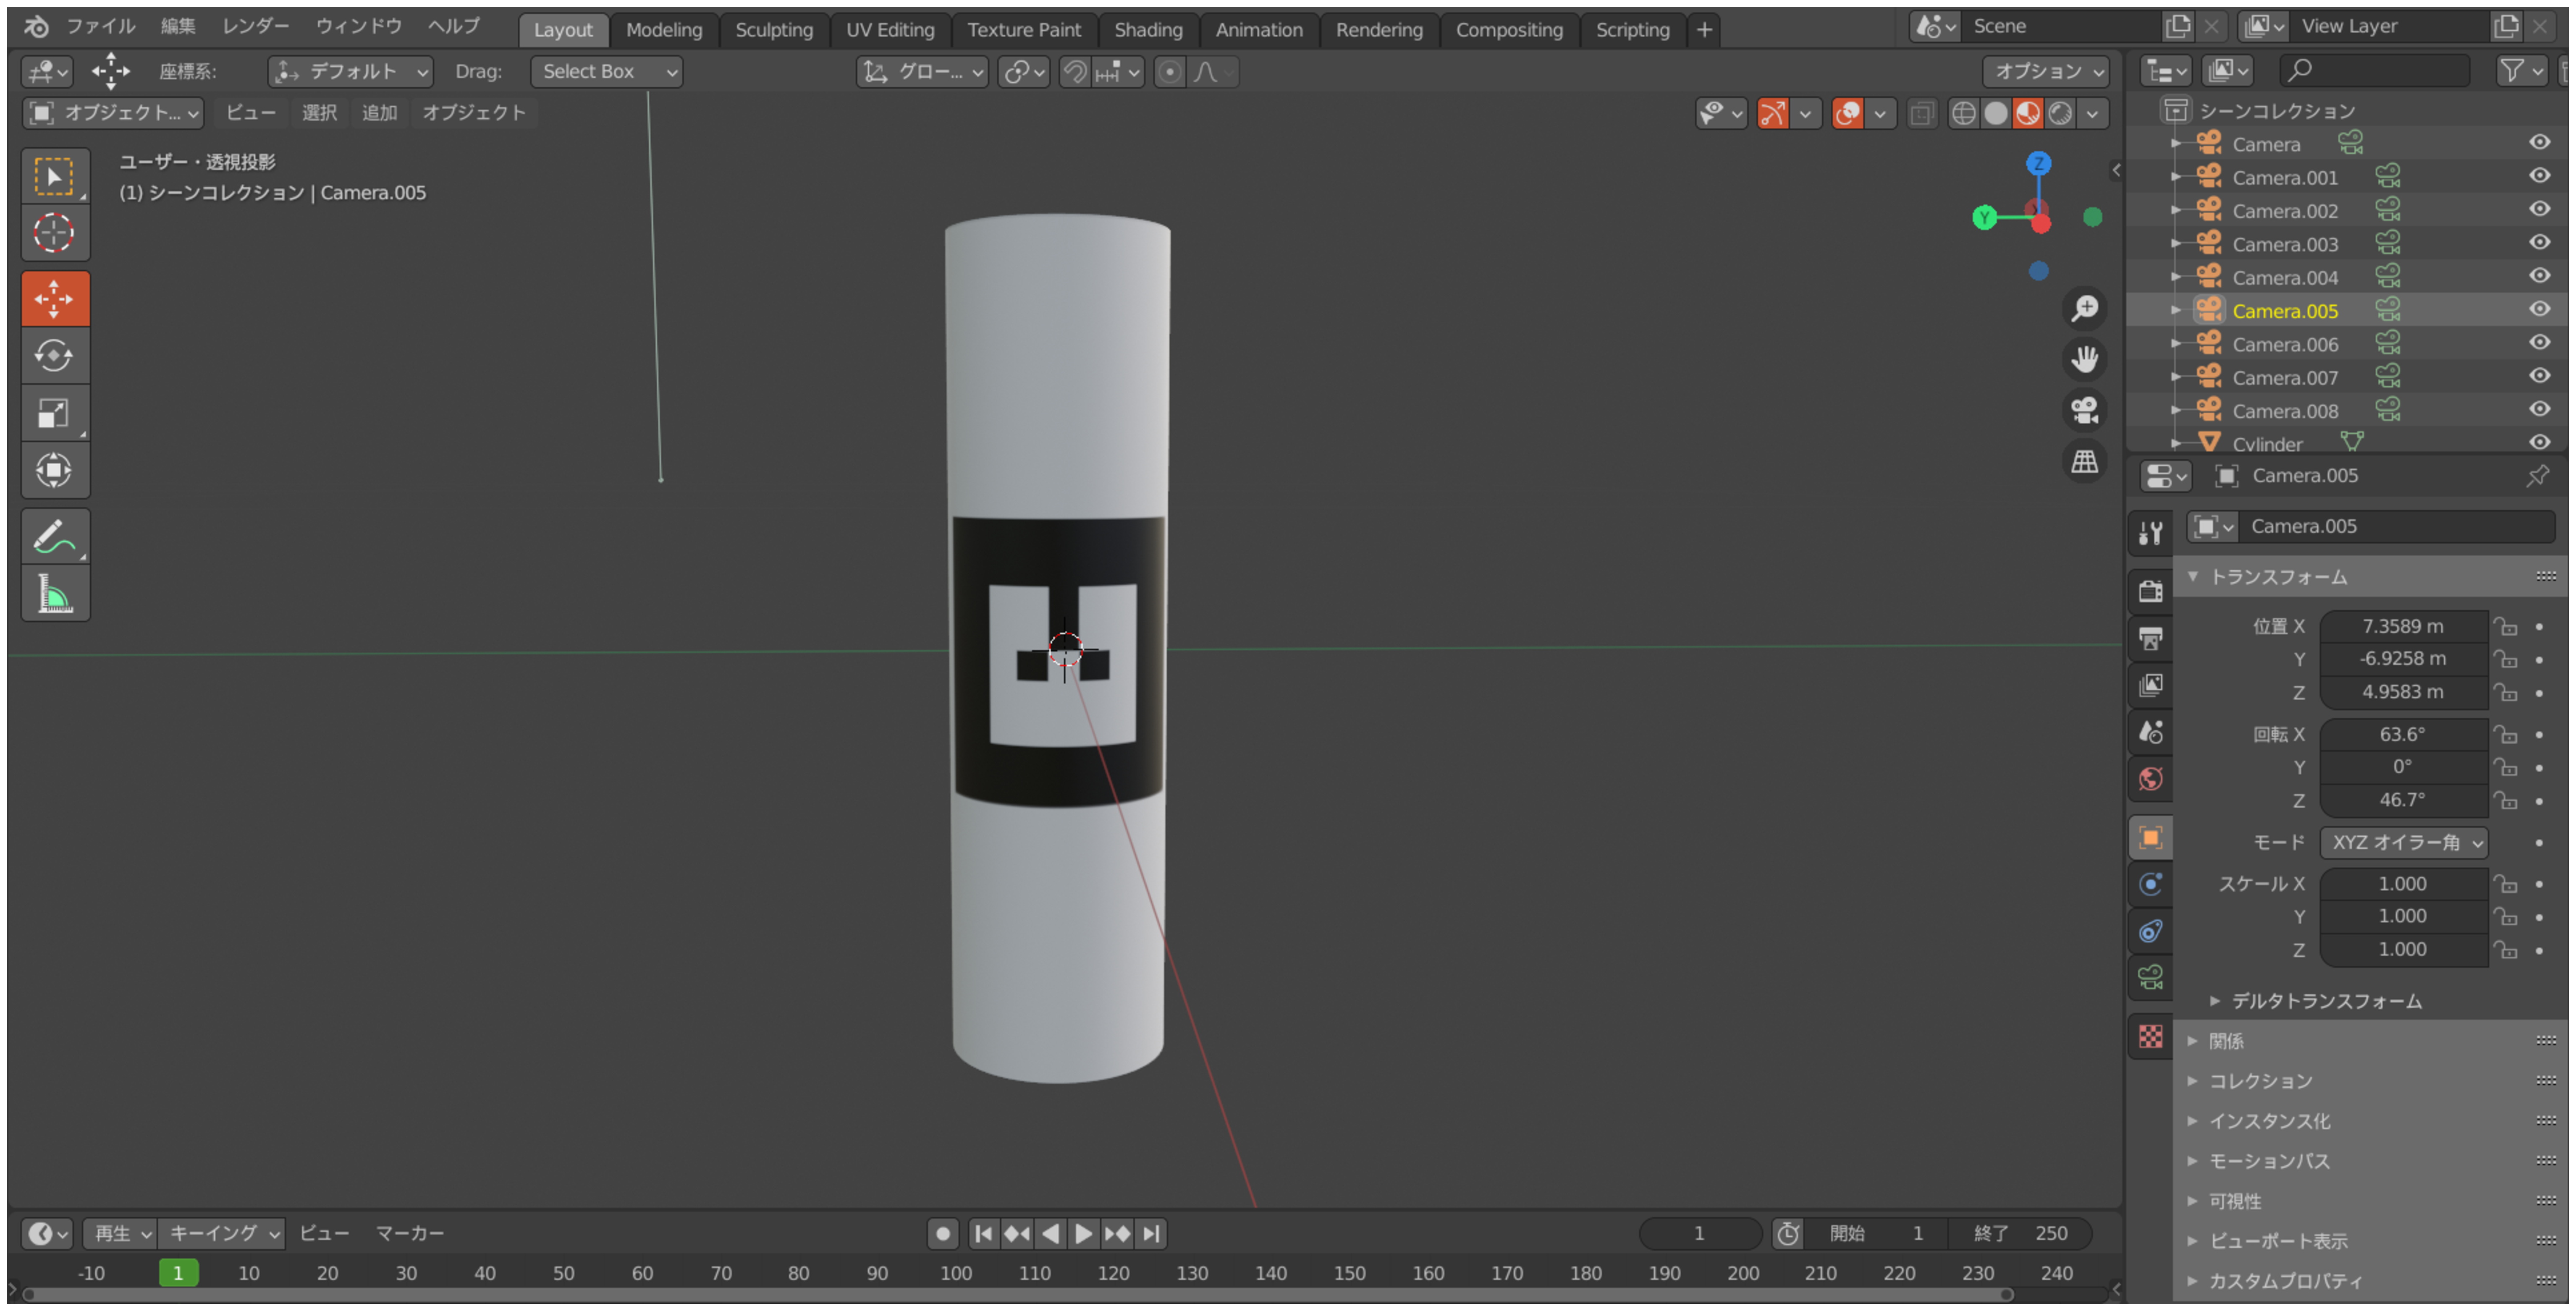
\includegraphics[width=90mm]{figure/eps/bl4.eps}
      \caption{変形ARマーカの完成図.}
      \label{bl4}
      \end{center}
      \end{figure}



この手順で,円柱に貼られたマーカを半径3種類とID10種類の合計30種類のモデルを作成する.また,平面状ARマーカの30種類も同様の手順で板にマーカを張り付け円柱と結合を行い作成する.




\subsection{学習用画像の撮影}
学習用画像は,変形ARマーカモデルと平面状ARマーカモデルをgazebo\cite{ga}の環境を用いて撮影を行う.
カメラは座標(0,0,0.5)の位置に設置し,画像サイズ(1920$\times$1080)で撮影を行う.
モデルの背景には,変形ARマーカは後で背景画像を合成できるように赤色の板を設置,平面状ARマーカの背景には白色の板を設置する.このままの環境では暗いためuser\_point\_lightを座標位置(x,y,z)がそれぞれ(1,1,1.2),(1,1,0.8),(0,0,1.2),(0,0,0.8),(1,-1,1.2),(1,-1,0.8)で配置を行い,壁が均一な明るさとなるよう撮影する.

変形AR マーカと平面状ARマーカのIDと半径が同じ種類をセットとなるように.それぞれ別のファイルに姿勢と名前が同じとなるように保存していく.変形ARマーカは(0,0,0.015)の位置を中心に(x,y,z)が最小値(0.3,-0.24,0.35)から最大値(0.8,0.24,0.65)の範囲に出現するように設定し,平面状ARマーカは(x,y,z)が(0.8,0,0.5)の位置に配置する.
ARマーカの姿勢はマーカが半分以上見える回転範囲[roll0~360°,pitch-35~35°,yaw-15~15°]に設定して撮影を行う.
撮影後,変形ARマーカの背景にテクスチャの合成を行う.
それぞれの画像をARマーカが写る位置でトリミングを行い,128$\times$128にリサイズをする.学習用に用意した同じ姿勢の変形ARマーカと平面状ARマーカの画像を図\ref{hennkei}図\ref{heimen}に示す.1種類あたり,1500枚ずつ用意する.訓練データ教師データ合わせて60種類$\times$1500枚の合計90000枚の画像を用意する.
















%----------------------------------------------


%----------------------------------------------
\chapter{評価実験}
\label{chap:4}
本章では,本手法の有効性を記すための評価実験について示す.

\section{実験概要}
SSDにより検出された変形ARマーカの姿勢推定を仮定して,評価を行う.
提案手法をバッチサイズ100,エポック数500で学習を行い変形ARマーカID0~9を平面への復元を行い
ID0の変形ARマーカを使用して姿勢推定を行う.
学習データ,データベース,推論データは,第2章で作成したものを使用する.
姿勢推定で用いる推論データは姿勢が分かるように姿勢情報を保存したものを用いる.
半径20,30,40mmの円柱それぞれ
100枚の背景テクスチャ付き変形ARマーカをランダム姿勢
で撮影した画像を使用する.
それぞれの推論結果は平均絶対誤差(MAE)を用いて推定された姿勢と正解姿勢の誤差を求める.
推論結果の平均のroll,pitch,yaw,平均誤差の4項目を求めて確認する.
MAEとは平均絶対2乗誤差の事であり2つのデータの誤差を絶対値で求め平均を取る誤差の指標である.
この実験で本手法による変形ARマーカの姿勢推定の精度を確認する.
なお,ここでの姿勢の角度は度数法によって表現する.

\newpage

\section{実験環境}
実験環境を表\ref{tab:kankyo}に示す.

\begin{table}[h]
  \centering
  \caption{実験環境}
    \begin{tabular}{c||c} \hline
    	OS & Ubuntu16.04 LTS \\ \hline
    	CPU &  Intel® Core™ i7-8700K CPU @ 3.70GHz × 12 \\ \hline
    	GPU & GeForce GTX 1080/PCle/SSE2 \\ \hline
     メモリ & 15.6 GiB \\ \hline
    	Python & 3.5.2 \\ \hline
    	Pytorch & 1.3.1 \\ \hline
  \end{tabular}
 \label{tab:kankyo}
\end{table}


\section{実験結果}

\subsection{提案手法による復元結果}
それぞれのID に対して,左から正解画像,変形ARマーカ画像,復元画像である.

\begin{itemize}
\item ID0
\end{itemize}

ID0の復元画像の出力結果を図\ref{i0}に示す.

      \begin{figure}[htbp]
      \begin{center}
      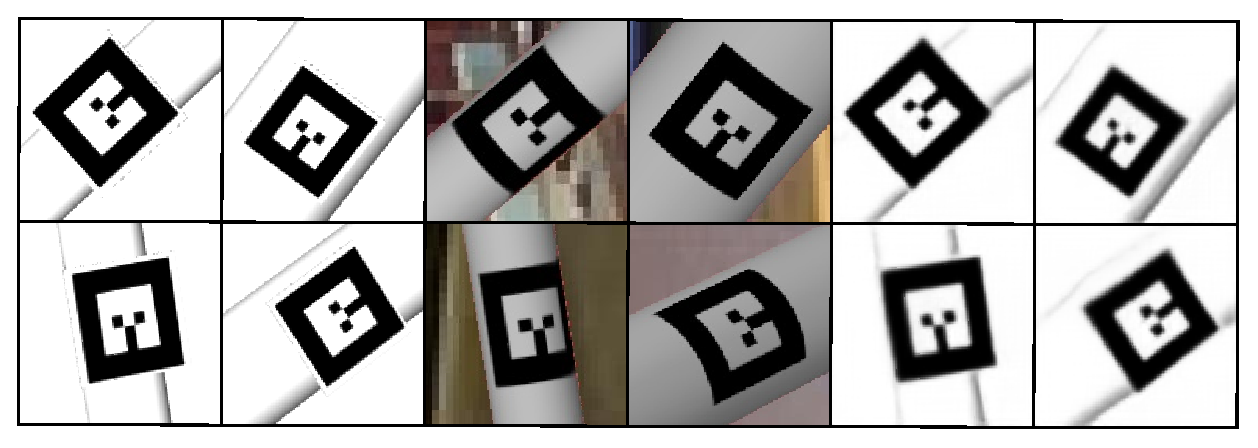
\includegraphics[width=85mm]{figure/eps/F0.eps}
      \caption{ID0の復元結果.}
      \label{i0}
      \end{center}
      \end{figure}
\newpage

\begin{itemize}
\item  ID1
\end{itemize}

ID1の復元画像の出力結果を図\ref{i1}に示す.

      \begin{figure}[htbp]
      \begin{center}
      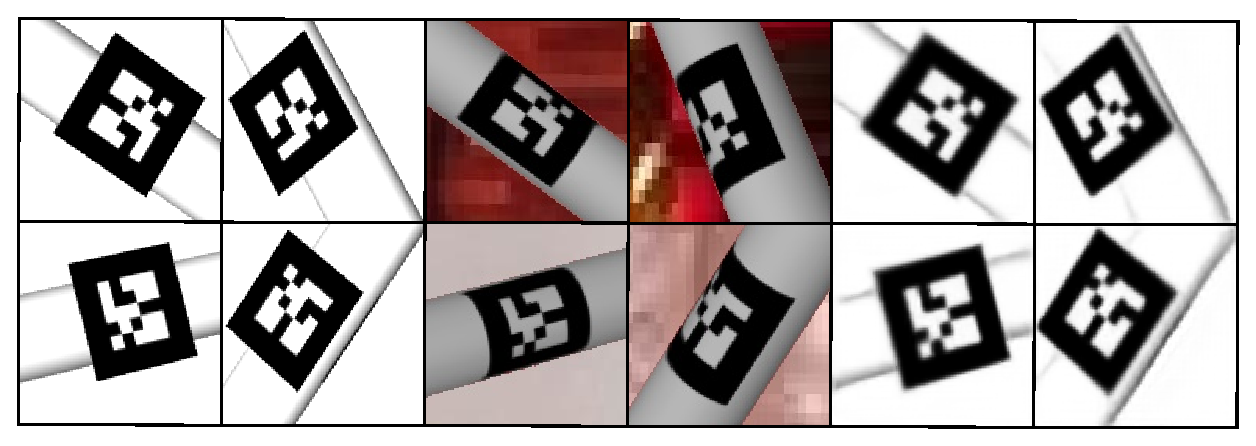
\includegraphics[width=85mm]{figure/eps/F1.eps}
      \caption{ID1の復元結果.}
      \label{i1}
      \end{center}
      \end{figure}


\begin{itemize}
\item  ID2
\end{itemize}

ID2の復元画像の出力結果を図\ref{i2}に示す.

      \begin{figure}[htbp]
      \begin{center}
      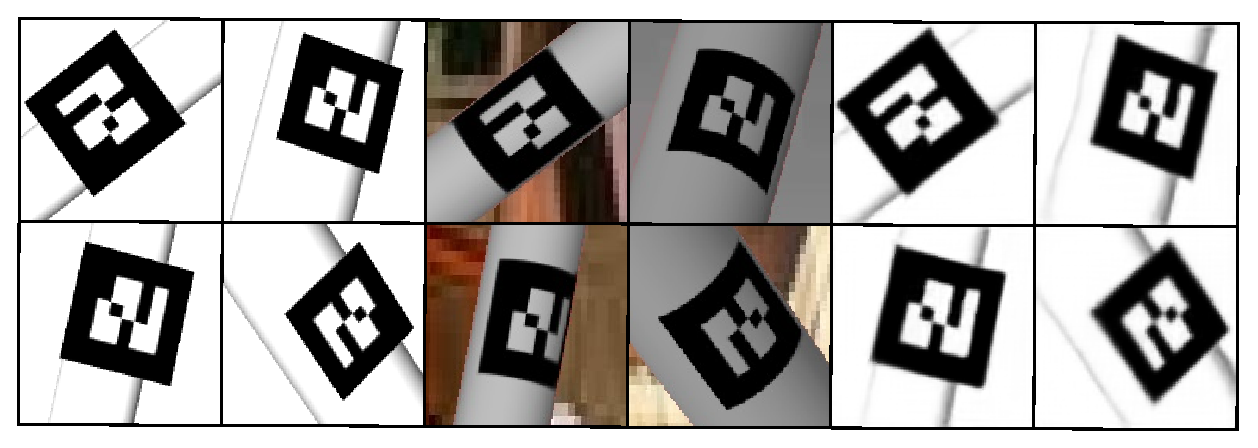
\includegraphics[width=85mm]{figure/eps/F2.eps}
      \caption{ID2の復元結果.}
      \label{i2}
      \end{center}
      \end{figure}


\begin{itemize}
\item  ID3
\end{itemize}

ID3の復元画像の出力結果を図\ref{i3}に示す.

      \begin{figure}[htbp]
      \begin{center}
      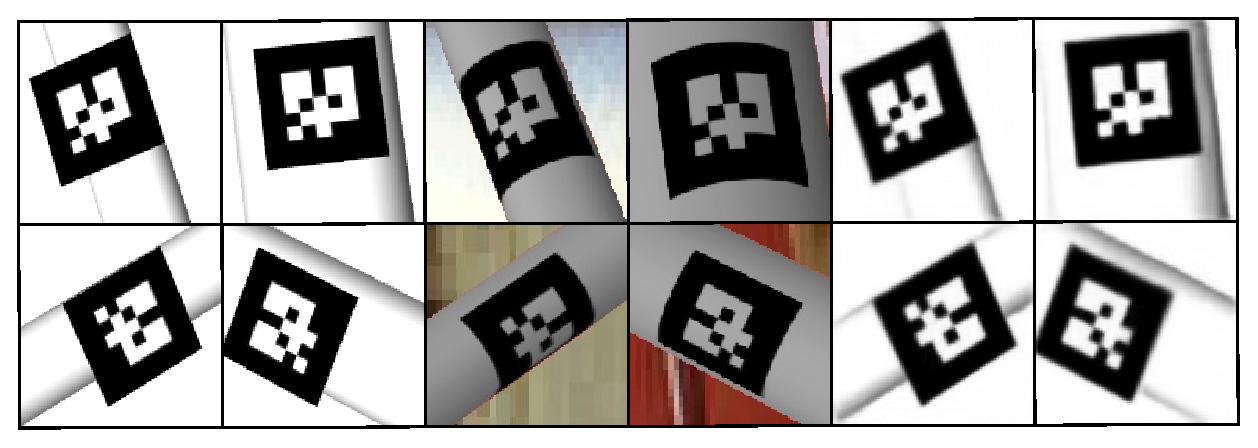
\includegraphics[width=85mm]{figure/eps/F4.eps}
      \caption{ID3の復元結果.}
      \label{i3}
      \end{center}
      \end{figure}

\newpage

\begin{itemize}
\item ID4
\end{itemize}

ID4の復元画像の出力結果を図\ref{i4}に示す.

      \begin{figure}[htbp]
      \begin{center}
      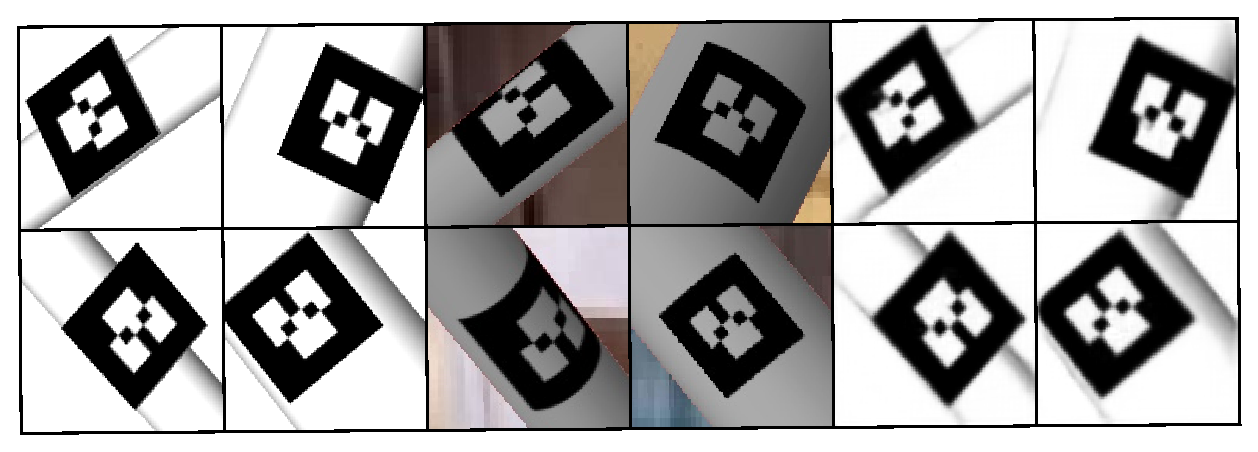
\includegraphics[width=85mm]{figure/eps/F5.eps}
      \caption{ID4の復元結果.}
      \label{i4}
      \end{center}
      \end{figure}


\begin{itemize}
\item  ID5
\end{itemize}

ID5の復元画像の出力結果を図\ref{i5}に示す.

      \begin{figure}[htbp]
      \begin{center}
      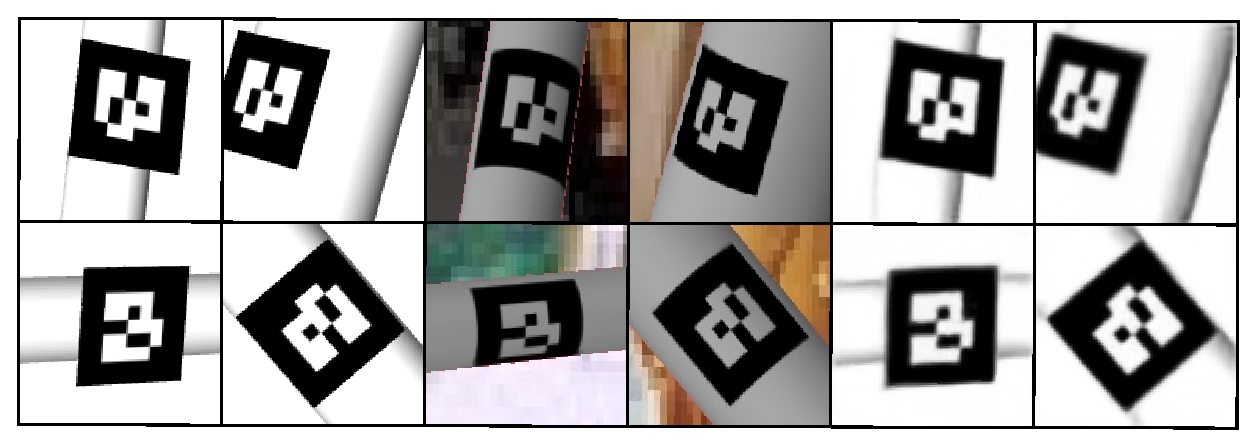
\includegraphics[width=85mm]{figure/eps/F6.eps}
      \caption{ID5の復元結果.}
      \label{i5}
      \end{center}
      \end{figure}



\begin{itemize}
\item  ID6
\end{itemize}

ID6の復元画像の出力結果を図\ref{i6}に示す.

      \begin{figure}[htbp]
      \begin{center}
      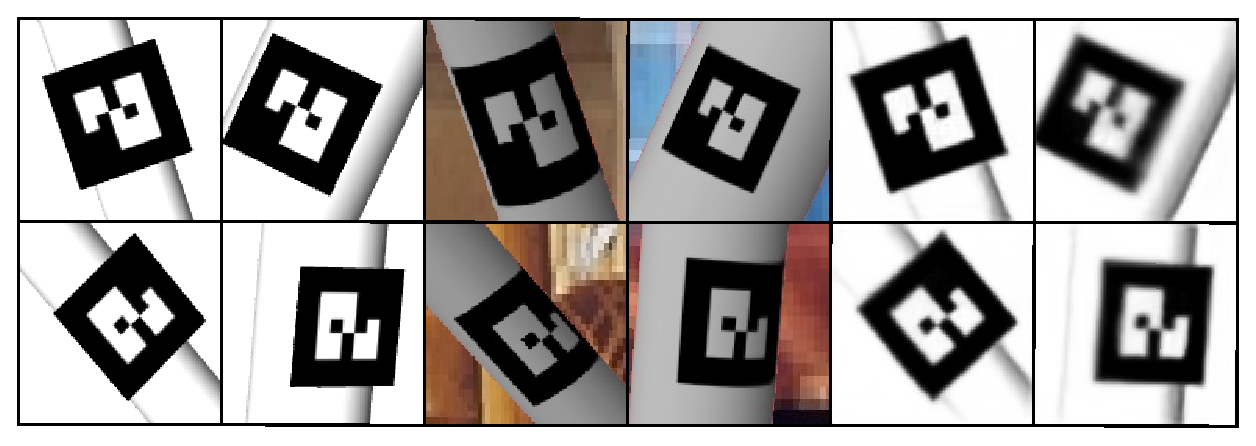
\includegraphics[width=85mm]{figure/eps/F7.eps}
      \caption{ID6の復元結果.}
      \label{i6}
      \end{center}
      \end{figure}

\newpage
\begin{itemize}
\item  ID7
\end{itemize}

ID7の復元画像の出力結果を図\ref{i7}に示す.

      \begin{figure}[htbp]
      \begin{center}
      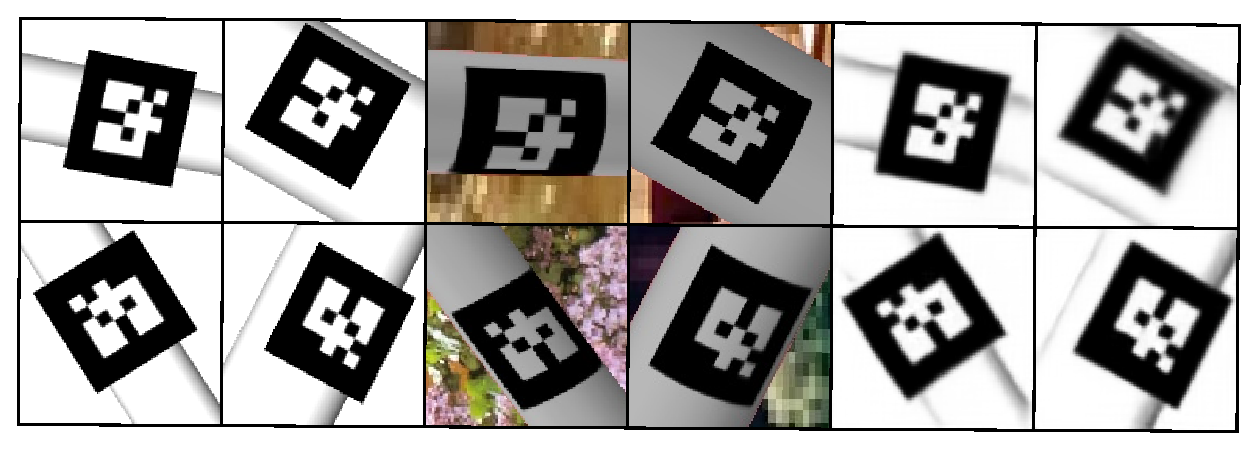
\includegraphics[width=85mm]{figure/eps/F8.eps}
      \caption{ID7の復元結果.}
      \label{i7}
      \end{center}
      \end{figure}



\begin{itemize}
\item  ID8
\end{itemize}

ID8の復元画像の出力結果を図\ref{i8}に示す.

      \begin{figure}[htbp]
      \begin{center}
      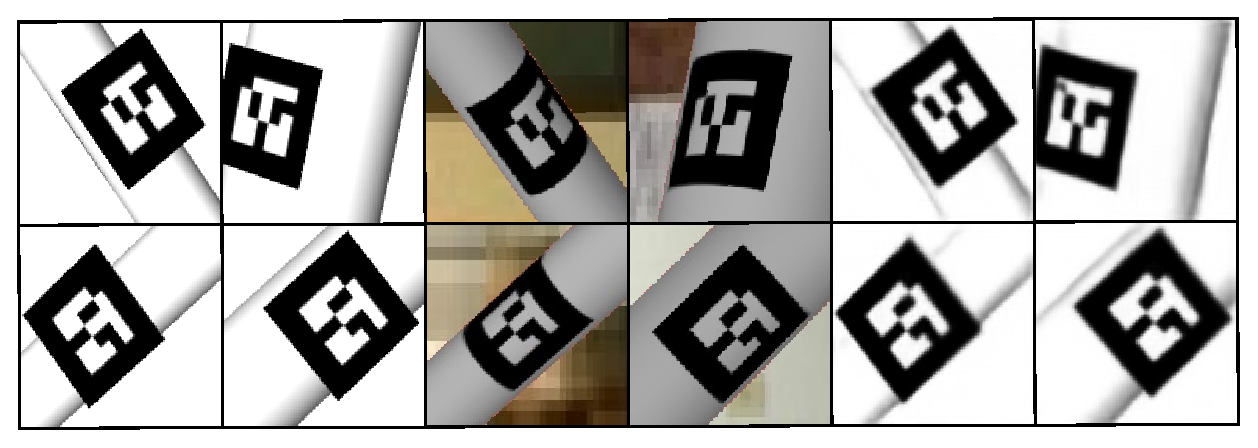
\includegraphics[width=85mm]{figure/eps/F9.eps}
      \caption{ID8の復元結果.}
      \label{i8}
      \end{center}
      \end{figure}


\begin{itemize}
\item  ID9
\end{itemize}

ID9の復元画像の出力結果を図\ref{i9}に示す.

      \begin{figure}[htbp]
      \begin{center}
      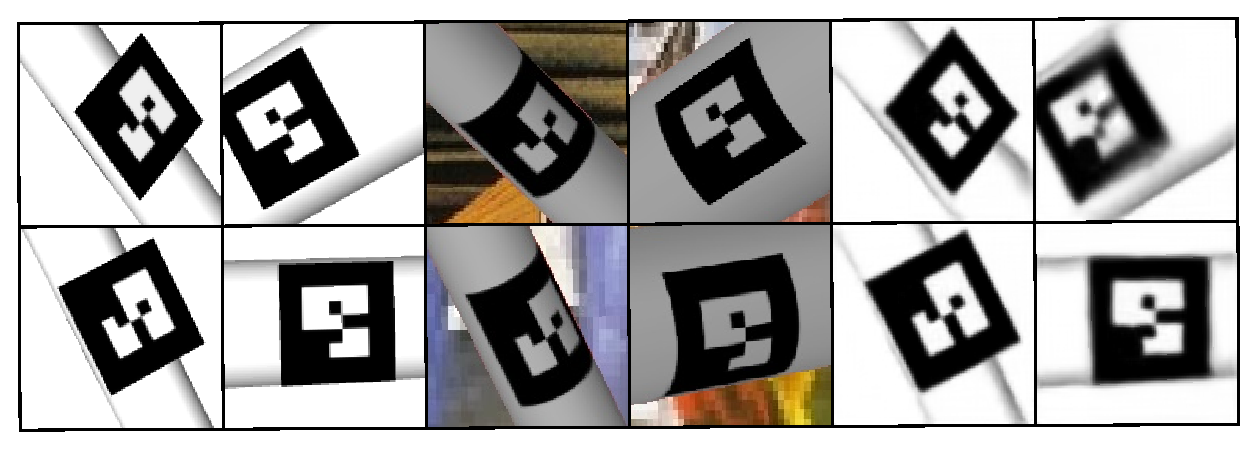
\includegraphics[width=85mm]{figure/eps/F10.eps}
      \caption{ID9の復元結果.}
      \label{i9}
      \end{center}
      \end{figure}


\subsection{提案手法を用いた姿勢推定結果}
提案手法により推定された各円柱半径における推論データ100枚の
roll,pitch,yaw,姿勢全体におけるMAEを表\ref{hyouka}に示す.



\begin{table}[h]
        \vspace{0zh}
          \begin{center}
            \caption{提案手法における姿勢推定の精度}
            \label{hyouka}
            \begin{tabular}{c|c|c|c|c} \hline
              円柱半径[mm]   & roll& pitch & yaw&姿勢全体 \\ \hline
              20& 5.30 & 3.64 & 3.42&4.12 \\ \hline
              30&5.78 & 4.49 & 3.71& 4.66 \\ \hline
              40&6.52 &4.51  &3.71&4.91 \\ \hline
              \end{tabular}
          \end{center}
        \vspace{-1.0zh}
\end{table}





\section{考察}
表\ref{hyouka}より,姿勢推定誤差のMAEは平均4~5前後の誤差という結果となり,半径の小さいARマーカほど推定結果がよくなっている.これは円柱の半径が小さいほど姿勢ごとに画像の特徴量が大きく変わるため,潜在変数が明確になるという事がこの結果の要因である.また,データベースの分解能を3度で用意したことにより,類似度計算を行う際にまったく同じ姿勢データがあると限らなかった.その為,推定誤差が生じるという結果になった.データベースの分解能を1度に設定し用意しておくことで範囲内の姿勢であればすべての角度に対応出来るため推定精度が上がると考えられる.

復元結果で示したように,提案手法による復元は行えているが,明確に表現されていない部分もある.今回は学習画像を1種類あたり1500枚で行ったが,学習画像のバリエーションを増やすことで変形ARマーカの潜在変数をより明確に取得することが可能となる.その為学習のバリエーションを増やすことで,復元精度・推定精度はともに高くなると考えられる.

















%----------------------------------------------


%----------------------------------------------
\chapter*{おわりに}
\label{chap:10}
\markboth{おわりに}{}
\addcontentsline{toc}{chapter}{おわりに}
本研究では,機械学習を用いたARマーカの位置姿勢推定を提案し,評価実験より,
機械学習によって変形したARマーカの姿勢を推定できることを確認した.
今後は復元精度と姿勢推定の精度の向上を考えた学習方法と,現実空間においてリアルタイム
での復元及び姿勢推定する方法の研究を行う予定である.
%----------------------------------------------



%%%%%%%%%%%%%%%%%%%%%%%%%%%%%%%%%%%%%%%%%%%%%%%%%%%%%%%%%%%%%%%%
\chapter*{謝 辞}
\markboth{謝 辞}{}
\addcontentsline{toc}{chapter}{謝  辞}
本研究を行うにあたり,終始懇切なるご指導を頂きました中部大学工学部 山内悠嗣教授に謹んで感謝します.
本研究において,助言や相談,実験データ取得に協力して頂いた機械知能研究室の皆様に感謝致します.
%%%%%%%%%%%%%%%%%%%%%%%%%%%%%%%%%%%%%%%%%%%%%%%%%%%%%%%%%%%%%%%%
\cleardoublepage
\markboth{参考文献}{}     %% BibTeX を使う
%\bibliographystyle{jalpha}
%\newcommand{\noop}[1]{}
%\bibliographystyle{jabbrv}
\bibliographystyle{junsrt}
\bibliography{reference}
%\nocite{*}
%\bibliography{./ref}


%%%%%%%%%%%%%%%%%%%%%%%%%%%%%%%%%%%%%%%%%%%%%%%%%%%%%%%%%%%%%%%%
%%% 必要に応じて付録を作る
%%%%%%%%%%%%%%%%%%%%%%%%%%%%%%%%%%%%%%%%%%%%%%%%%%%%%%%%%%%%%%%%
% \chapter*{付  録}
% \markboth{付  録}{}
% \addcontentsline{toc}{chapter}{付  録}

%%%%%%%%%%%%%%%%%%%%%%%%%%%%%%%%%%%%%%%%%%%%%%%%%%%%%%%%%%%%%%%%

%%%%%%%%%%%%%%%%%%%%%%%%%%%%%%%%%%%%%%%%%%%%%%%%%%%%%%%%%%%%%%%%
%%% 必要に応じて論文目録を作る
%%%%%%%%%%%%%%%%%%%%%%%%%%%%%%%%%%%%%%%%%%%%%%%%%%%%%%%%%%%%%%%%



%%%%%%%%%%%%%%%%%%%%%%%%%%%%%%%%%%%%%%%%%%%%%%%%%%%%%%%%%%%%%%%%

\backmatter         %%% 奥付
\thispagestyle{empty}
\vspace*{18cm}
\begin{flushright}
\begin{tabular}{r}
\Hline
%\large
{機械学習を用いた変形ARマーカの位置姿勢推定}\\
(中部大学工学部ロボット理工学科)\\
ER17076\\
安井 理\\
2021年 2月12日\\ %(卒業研究発表会の日時とする)

\Hline
\end{tabular}
\end{flushright}
\end{document}